% !TEX program = pdflatex --shell-escape

\documentclass[11pt]{article}
\usepackage[round,sort&compress,semicolon]{natbib}
\usepackage{times}
\usepackage[T1]{fontenc}
\usepackage[utf8]{inputenc}
\usepackage[pdftex]{graphicx}
\usepackage[letterpaper, left=1.0in, right=1.0in, top=1.0in, bottom=1.0in]{geometry}
\usepackage{ragged2e}
\usepackage{url}
\usepackage{setspace}
\usepackage{lineno}
\usepackage{multirow}
\usepackage{pdflscape}
\usepackage[backref=page]{hyperref}
\usepackage{hyperref}
\usepackage{rotating}
\usepackage{booktabs}
\usepackage[hypcap, labelsep=period, labelfont=bf]{caption}
\usepackage{array}
\usepackage{color}
\usepackage{soul}
\usepackage{mathtools}
\usepackage{pdflscape}
\usepackage[normalem]{ulem}

\usepackage{amsmath}
\usepackage{amsfonts}       % blackboard math symbols
\usepackage{nicefrac}       % compact symbols for 1/2, etc.
\usepackage{microtype}      % microtypography
\usepackage{lipsum}		% Can be removed after putting your text content
\usepackage{doi}

% can be used for revision to outline revised figures in a red-box
% \usepackage{efbox,graphicx}
% \efboxsetup{linecolor=red,linewidth=2pt}


\usepackage[usenames,dvipsnames,svgnames,table]{xcolor}
\urlstyle{same}
\setlength{\RaggedRightParindent}{\parindent}
\linenumbers
\linespread{1.15}

% restart counting in the supplement
\newcommand{\beginsupplement}{%
	\setcounter{table}{0}
	\setcounter{figure}{0}
	% \setcounter{section}{0}
	% \setcounter{subsection}{0}	
	\renewcommand{\thetable}{S\arabic{table}}%
	\renewcommand{\thefigure}{S\arabic{figure}}%
	% \renewcommand{\thesection}{S\arabic{section}}%
	% \renewcommand{\thesubsection}{S\arabic{section}.\arabic{subsection}}%          
}

%%% Add PDF metadata to help others organize their library
%%% Once the PDF is generated, you can check the metadata with
%%% $ pdfinfo template.pdf
\hypersetup{
     colorlinks   = true,
     citecolor    = Indigo,
     linkcolor    = DarkCyan,
	pdftitle = {Estimating Waiting Distances Between Genealogy Changes under a 
		Multi-Species Extension of the Sequentially Markov Coalescent},
	pdfsubject = {Evolutionary biology},
	pdfauthor = {Patrick F. ~McKenzie},
	pdfkeywords = {Recombination, Phylogeny, SMC, Gene Tree, Species Tree, Concatalescence, ARG},
}

% \renewcommand{\shorttitle}{MSC Waiting Distance Distribution}

\begin{document}

\begin{center}
	{\bf \Large
		Estimating Waiting Distances Between Genealogy Changes under a \\[0.25cm]
		Multi-Species Extension of the Sequentially Markov Coalescent
	}\\[0.5cm]

	Patrick F. McKenzie$^{1}$ and Deren A. R. Eaton$^{1, *}$\\[0.25cm]

	\emph{
	$^{1}$ Department of Ecology, Evolution, and Environmental Biology, Columbia University, New York, NY 10027, USA\\[0.5cm]
	$^{*}$ Contact: de2356@columbia.edu\\[0.5cm]
	}
\end{center}

% keywords can be removed
Keywords: Recombination, Phylogeny, SMC, Gene Tree, Species Tree, Concatalescence, ARG

\RaggedRight

%\section*{Significance Statement}
%Genealogical relationships vary spatially along genomes as a result of coalescent
 %variation and recombination through time. These spatial genealogical patterns 
 %contain rich information about the evolutionary history of populations but are 
 %difficult to reconstruct from sequence data. Here, we extend recently developed 
 %theory for predicting the genomic interval lengths between changes in 
 %genealogical trees (different coalescent times) or topologies (different 
 %coalescent times and relationships). Our solutions allow for calculating 
 %these “waiting distances” within the context of a parameterized species tree 
 %model. This new framework, termed the MS-SMC, provides a link between the 
 %multispecies coalescent (MSC) and the sequentially Markov coalescent (SMC), 
 %paving the way for new spatial phylogenetic inference methods capable of 
 %analyzing linked genome data.

\section*{Abstract}
Genomes are composed of a mosaic of segments inherited from different ancestors, 
each separated by past recombination events. Consequently, genealogical
relationships among multiple genomes vary spatially across different genomic 
regions. 
Genealogical variation among unlinked 
(uncorrelated) genomic regions is well described for either a single 
population (coalescent) or multiple structured populations (multispecies coalescent).
However, the expected similarity among genealogies at linked regions of a 
genome is less well characterized. 
Recently, an analytical solution was derived for 
the distribution of the waiting distance for a change in the genealogical tree 
spatially across a genome for a single population with constant effective 
population size. Here we describe a generalization of this 
result, in terms of the 
distribution of waiting distances between 
changes in genealogical trees and topologies for multiple structured populations
with branch-specific effective population sizes (i.e., under the multispecies 
coalescent). 
We implemented our model in the Python package \emph{ipcoal} and validated its
accuracy against stochastic coalescent simulations. Using a novel
likelihood framework we show that tree and topology-change waiting distances
in an ARG can be used to fit species tree model parameters, demonstrating an
application of our model for developing new methods for phylogenetic inference.
The Multi-Species Sequentially Markov Coalescent (MS-SMC) model presented here
represents a major advance for linking local ancestry inference to hierarchical
demographic models.


\section{Introduction}
The multispecies coalescent (MSC) is an extension of the coalescent 
\citep{kingman1982coalescent}, a model that describes the distribution of genealogical 
histories among gene copies from a set of sampled individuals. Whereas the 
coalescent models a single panmictic population, the MSC includes constraints that prevent 
samples in different lineages from sharing a most recent genealogical ancestor until prior
to a population divergence event that separates them \citep{maddison1997gene,maddison2006inferring}. 
Conceptually, the MSC can be viewed as a piecewise model composed of the standard
coalescent applied to each interval of a "species tree" representing the relationships
and divergence times among isolated lineages. Genealogies are constrained to be
embedded within species trees, 
and the joint likelihood of 
MSC model parameters can be calculated from the coalescent times among a 
distribution of sampled genealogies
\citep{rannala2003bayes,degnan2009gene}. In both the coalescent
and MSC models, effective population size ($N_e$) is the key parameter determining 
the rate of coalescence and can vary across different lineages. 


Importantly, both the single-population coalescent and the MSC specify 
the distribution of \emph{unlinked} (uncorrelated) genealogies.
By contrast, two linked genealogies that are drawn from nearby regions of a genome %the genome 
are expected to be more similar than two random draws under these models. This spatial 
autocorrelation is a consequence of shared ancestry among samples at nearby regions, 
which decays over time and distance as recombination events reduce their shared ancestry.
To be clear, the spatial correlation here refers to the similarity 
among neighboring genealogies on a chromosome, and not to the similarity of genomes 
in geographic space.
As a data structure, an ordered series of linked genealogies and the lengths of 
their associated intervals on a chromosome (Fig.~\ref{fig:ARG-cartoon}) is represented 
by an ancestral recombination graph (ARG)
\citep{griffiths_ancestral_1996,lewanski_era_2024,y_c_brandt_evaluation_2022,nielsen_inference_2025,wong_general_2024},
or similarly, a tree-sequence 
\citep{kelleher2016efficient}
(hereafter we will refer to it generically as an ARG).

An algorithm to stochastically generate ARGs under the coalescent with 
recombination was developed early on by \citet{hudson1983properties} and 
later extended as a spatial algorithm by \citet{wiuf_recombination_1999}.
This latter process models the difference between sequential 
genealogies by randomly detaching an edge from a genealogy and sampling
a waiting time (based on the 
coalescent rate) until it reconnects to the genealogy at a different shared ancestor.
Thus, under this spatial model, a set of samples effectively substitutes
one ancestor for another on either side of each recombination breakpoint.
Implicit to this algorithm is the assumption that recombination 
occurs at some predictable rate (or rate map) from which the 
waiting distance between recombination events can be modeled as an 
exponentially distributed random variable \citep{wiuf_recombination_1999}.
Although generating ARGs consistent with a demographic model is 
relatively simple under this process, inferring an ARG from sequence data 
-- composing a set of recombination breakpoints and local genealogy inferences -- 
remains highly challenging \citep{y_c_brandt_evaluation_2022}.
This stems in part from the great complexity of this problem 
but also reflects limitations of our current models for 
extracting historical information from linked genome data.

A major advance was achieved through development of the sequentially Markov 
coalescent (SMC), a simpler approximation of the coalescent with recombination
that restricts the types of recombination events that can occur 
\citep{mcvean2005approximating}. Specifically,
an edge that is detached from a genealogy by recombination is allowed only to
re-coalesce with ancestral lineages that contributed genetic material to samples
in that interval (as opposed to re-coalescing with any ancestral lineage). 
This greatly reduces the space of possible ARGs without changing the
distribution of sequential genealogies, and in doing so it enables modeling
changes between sequential genealogies
as a Markov process \citep{mcvean2005approximating}. 
Under these assumptions a tractable likelihood framework can be developed. 
Because neither genealogies nor segment lengths can
be observed directly, most SMC-based inference methods use 
a hidden Markov model (HMM) to treat these as hidden states 
that influence observable changes in sequence data \citep{spence_inference_2018}.
Examples of inference tools built on the SMC framework include 
PSMC \citep{li2011inference} and MSMC \citep{schiffels_inferring_2014}
which use pairwise coalescent times between sequential genealogies
to infer changes in effective population sizes through time, 
and ARGweaver \citep{rasmussen2014genome, hubisz2020inference} 
or SINGER \citep{deng_robust_2024},
which infer ARGs from genome alignments using SMC-based conditional sampling methods.

\begin{figure}[t]
	\centering
	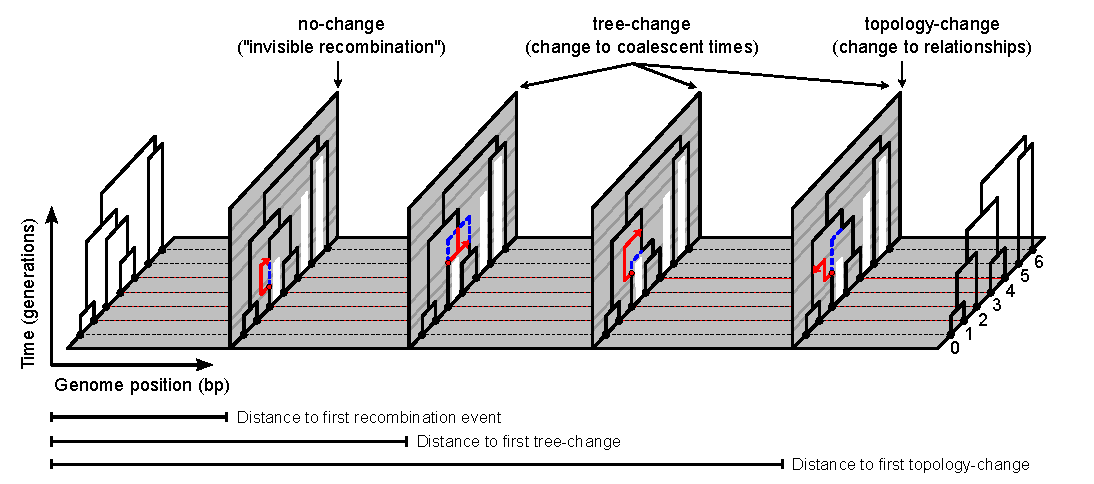
\includegraphics[width=0.99\textwidth]{figures/current/Fig1-recomb-types-on-ARG.pdf}
	\caption{
		An ancestral recombination graph (ARG)
		is composed of a series of genealogies each spanning non-overlapping 
		intervals of a genome separated by recombination breakpoints. Here, 
		four recombination breakpoints separate interval
		start and end positions along a small chromosome alignment. 
		The individual genealogies represent the history of a set of 7 samples
		constrained by a 4-tip species tree model (as in Fig.~2).
		Recombination events are indicated by vertical panels. Each shows the SMC' process by 
		which a subtree (below the red circle) is detached and then re-coalesces (red arrow)
		with one of the remaining lineages.
		The former edge (blue dotted) which existed throughout the interval to the left of a 
		panel is replaced by a new edge (red) through the subsequent interval. 
		Vertical bars 
		(white) represent barriers to coalescence between samples in different species
		tree intervals (MSC model lineages).
		Four categories of recombination events are shown from left to right, representing
		different outcomes based on the lineage with which a detached subtree re-coalesces.
		These are grouped more generally into 
		three \emph{event types}: (1) no-change, (2) tree-change, and (3) topology-change.
		Every recombination event causes either a no-change or tree-change event, whereas
		topology-change events are a subset of possible tree-change events. The expected waiting
		distance until a specific recombination event type occurs can be calculated under 
		the MS-SMC given a starting genealogy, MSC model, and recombination rate.
	}
	\label{fig:ARG-cartoon}
\end{figure}


\cite{marjoram2006fast}
described an important extension to the SMC, termed the SMC', for additionally
modeling "invisible" recombination events, in which a detached lineage re-attaches
with its own ancestral lineage prior to the time of that lineage's next coalescent event. 
This leads to no change between the genealogies in two sequential genomic intervals
despite the occurrence of a recombination event between them. The inclusion of
such events has been shown to 
significantly improve inference methods \citep{wilton2015smc}. 
Under the SMC', a detached lineage can thus re-coalesce with an allowable 
ancestral lineage over a continuous range of time, leading to one of 
four possible categorical patterns for the relationship between two
sequential genealogies
(Fig.~\ref{fig:ARG-cartoon}, Fig.~\ref{fig:figS-recomb-types}):
(1) no change;
(2) shortening of a coalescent time; (3) lengthening of a coalescent time; 
and (4) a change to the genealogical topology (relationships).
These can be grouped more generally into three types: 
"no-change" (category 1), "tree-change" (categories 2-4), and "topology-change"
(category 4). Recently, \citet{deng_distribution_2021} derived a set of 
solutions for the waiting distances to each of these three types of 
outcomes for a single population with constant effective population size.
This provided an important advance by establishing a neutral expectation 
not only for the distance until the next recombination event occurs, 
but more specifically, for the distance until different categorical types
of recombination events occur. Such events leave different detectable 
signatures in sequence data and extend across different spatial distances 
of the genome, thus extending the scale over which information from 
spatial genealogical patterns can be extracted from genomes.


Here, we extend the theory of \citet{deng_distribution_2021} to an MSC framework
to derive the distribution of the waiting distance until different types of
genealogy changes occur under a parameterized species tree model.
The waiting distances between recombination events that cause topology-change 
may be of greatest interest, as they leave the most detectable signatures 
in sequence data and are relevant to expected gene tree distributions that form
an important component of many MSC-based methods \citep{
degnan2009gene, baum_concordance_2007, knowles_estimating_2011}.
The waiting distance between topology-change events may include multiple
intervening recombination events of the no-change or tree-change type
(Fig.~\ref{fig:ARG-cartoon}).
The relative occurrence of events that do not result in topology 
changes can be especially high in small sample sizes \citep{wilton2015smc}, 
which are common in MSC-type datasets in which samples are partitioned 
among species tree intervals. 
Since the partitioning of 
coalescent events among species tree intervals is expected to constrain 
the types of recombination events that will be observed, the
distributions of waiting distances between different types of 
genealogy changes should be highly dependent on, and thus informative about, 
the species tree model. We refer to the general framework of embedding the 
SMC' in an MSC model as the MS-SMC.


%%%%%%%%%%%%%%%%%%%%%%%%%%%%%%%%%%%%%%%%%%%%%%%%%%%%%%%%%%%%%%%%%%%%%%%%%%%
%%%%%%%%%%%%%%%%%%%%%%%%%%%%%%%%%%%%%%%%%%%%%%%%%%%%%%%%%%%%%%%%%%%%%%%%%%%
%%%%%%%%%%%%%%%%%%%%%%%%%%%%%%%%%%%%%%%%%%%%%%%%%%%%%%%%%%%%%%%%%%%%%%%%%%%
%%%%%%%%%%%%%%%%%%%%%%%%%%%%%%%%%%%%%%%%%%%%%%%%%%%%%%%%%%%%%%%%%%%%%%%%%%%
%%%%%%%%%%%%%%%%%%%%%%%%%%%%%%%%%%%%%%%%%%%%%%%%%%%%%%%%%%%%%%%%%%%%%%%%%%%
%%%%%%%%%%%%%%%%%%%%%%%%%%%%%%%%%%%%%%%%%%%%%%%%%%%%%%%%%%%%%%%%%%%%%%%%%%%
%%%%%%%%%%%%%%%%%%%%%%%%%%%%%%%%%%%%%%%%%%%%%%%%%%%%%%%%%%%%%%%%%%%%%%%%%%%
%%%%%%%%%%%%%%%%%%%%%%%%%%%%%%%%%%%%%%%%%%%%%%%%%%%%%%%%%%%%%%%%%%%%%%%%%%%
%%%%%%%%%%%%%%%%%%%%%%%%%%%%%%%%%%%%%%%%%%%%%%%%%%%%%%%%%%%%%%%%%%%%%%%%%%%
%%%%%%%%%%%%%%%%%%%%%%%%%%%%%%%%%%%%%%%%%%%%%%%%%%%%%%%%%%%%%%%%%%%%%%%%%%%


\section{Approach}
\subsection{Comparison to Deng \emph{et al.} (2021)} 

Our approach is a generalization of the \citet{deng_distribution_2021} derivation 
of waiting distances to genealogy changes for a single population of constant size. 
We modified the single-population model to (1) include barriers to coalescence imposed
by a species tree topology, and (2) integrate over changing coalescence rates along
paths through multiple species tree intervals with different effective population 
sizes. 
In addition, we introduce a novel application of our MS-SMC model, utilizing
a likelihood-based framework to estimate MSC model parameters from the waiting
distances between tree-change and topology-change events in an ARG.


\subsection{MSC model description}
Given an MSC model ($\mathcal{S}$) composed of a species tree topology with divergence
times ($W$) in units of generations and constant diploid effective population 
sizes ($N_e$) assigned to each branch, an embedded genealogy ($\mathcal{G}$) for 
any number of sampled gene copies ($k$) can be generated
by randomly sampling coalescent times at which to join two samples into a 
common ancestor, starting from samples at the present in each interval.
Following \citet{kingman1982coalescent}, the probability of a 
coalescent event one generation in the past (reducing the 
number of samples from $k$ to $k$-1) 
is given by equation 1. 
From this, we can model the waiting time ($t_k$) until the next coalescence 
event as an exponentially distributed random variable with rate parameter 
$\lambda_k$, and its expectation ($\mathbb{E}[t_k]$) as:
% 
% From this, we can model the expected 
% waiting time ($\mathbb{E}[t_k]$) until the next coalescence event as an 
% exponentially distributed random variable with rate parameter $\lambda_k$:

\begin{equation}
\begin{aligned}
	&\lambda_k = \mathbb{P}(\text{coal~event~} | N_e,k) = \frac{k(k-1)}{2N_e}
	\\
	&~~and:
	\\[0.15cm]
	&\mathbb{E}[t_k] = 1 / \lambda_k
	\\[0.15cm]	
\end{aligned}
\end{equation}

\noindent In a single population model
with constant $N_e$ the expected waiting time between coalescent events 
increases monotonically after each coalescent event, since the number of
remaining samples always decreases. In an MSC model, 
however, the expected waiting time between coalescence events can increase or 
decrease through time, as the transition from one population interval to another 
can be associated with a different $N_e$ value and an increase in the number 
of samples.

Based on this generative framework for sampling genealogies 
under a demographic model, 
the probabilities of observed genealogies can also be calculated under 
a demographic model.
The probability of a genealogy embedded in a single population model is
the product of the probability densities of each waiting time between 
coalescent events \citep{kingman1982coalescent}. 
The process is similar for a genealogy embedded in a species tree model, but
requires evaluating the probabilities of coalescent waiting times within each
species tree interval separately -- 
including the probability that all gene copies do not coalesce before the 
end of the interval \citep{rannala2003bayes}.
A key feature of this framework is that for each coalescent interval 
with $k$ gene copies and effective population size $N_e$, we can 
calculate the coalescent rate ($\lambda_k$) and use the exponential probability
density function (Equation 2) to evaluate the likelihood of the 
demographic model parameters based on the distributions of coalescent 
times in one or more genealogies.
	
\begin{equation}
	f(t_k; \lambda_k) = \lambda_k e^{-\lambda_k t_k}
\end{equation}


\subsection{MS-SMC model description and notation}
Under the SMC' model, sampling of a linked genealogy requires considering not only 
demographic model parameters, 
as we did above, but also an existing genealogy -- it is a method 
for sampling the next genealogy conditional on the previously observed one. 
If we define the previous genealogy as $\mathcal{G}$, and the sum of its edge lengths 
as $L(\mathcal{G})$, then under the assumption of a constant recombination rate through time,
a recombination break point can be uniformly sampled from $L(\mathcal{G})$ to occur with 
equal probability anywhere on $\mathcal{G}$. 
A recombination event creates a bisection on a branch, separating a subtree 
below the cut from the rest of the genealogy 
(Fig.~\ref{fig:ARG-cartoon}, Fig.~\ref{fig:figS-recomb-types}).
The subtree must then re-coalesce 
with an edge on the genealogy from which it was detached at a time
above the recombination event.
The waiting time until this re-coalescence event occurs is sampled 
stochastically 
using equation (1), where the expectation is determined by the 
number of samples and the effective population size.


In a single population model with constant $N_e$, the expected waiting time until 
re-coalescence increases monotonically with each coalescence event 
backwards in time, since each event decreases $k$.
Once again, the MSC model differs from this: 
coalescent events similarly decrease $k$, but the merging of 
species tree branches into ancestral intervals increases $k$, and $N_e$ 
can also vary among species tree intervals. 
Thus, the probability that a detached subtree re-coalesces to the genealogy 
can vary through time along its path of possible reconnection points through 
different species tree intervals.
To calculate these probabilities, a species tree and genealogy can be decomposed into a 
series of relevant intervals between events that change rates of coalescence,
which we refer to as the genealogy embedding table 
(Fig.~\ref{fig:embedding-table}).
From this table it is possible to calculate the probabilities of different
recombination event type outcomes and, consequently, to model the expected 
waiting distances until specific recombination event types occur. 


\begin{figure}[t]
	\centering
	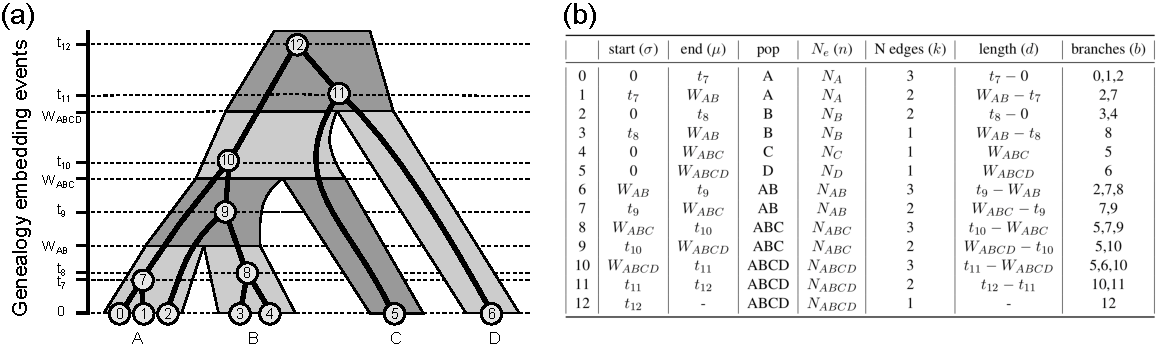
\includegraphics[width=0.99\textwidth]{figures/current/Fig2-embedding-table.pdf}
	\caption{
		An example genealogy embedded in a species tree and the corresponding
		embedding table used for MS-SMC calculations. 
		(a) A four tip species tree is composed of seven discrete population
		intervals separated by speciation events ($W_x$), each of which can be
		further dissected by coalescent events ($t_x$).
		(b) The probability of coalescence is constant within each discrete
		interval and is scaled by the number of lineages ($k$), the effective 
		population size ($n$), and the interval length ($d$).
		Under the MS-SMC, the probability that a detached lineage will re-coalesce
		on a specific branch of the genealogy (e.g., branch 7) is calculated using
		the piecewise constant probabilities from each discrete interval spanning
		that branch (e.g., rows 1, 6, 7, and 8 in the embedding table).
	}
\label{fig:embedding-table}
\end{figure}

Each interval of the genealogy embedding table contains a constant number
of genealogy branches ($k_i$) and a constant effective population size 
($n_i$) such that the rate of coalescence is also constant.
We define a number of additional variables related to this table. 
The length of each interval is $d_i$, and its lower and upper bounds 
are $\sigma_i$ and $\mu_i$, respectively. Similarly, the lower and upper 
bounds of a genealogy branch ($b$) are defined as $t_b^l$ and $t_b^u$, 
respectively. 
An indexing variable, $\mathcal{I}_b$, is defined as the
ordered set of intervals that are spanned by a specific branch
of an embedded genealogy. As an example, consider 
genealogy branch 7 from Fig.~\ref{fig:embedding-table}a.
This branch spans four intervals, 
labeled as rows 1, 6, 7, and 8 in
the associated genealogy embedding table
(Fig.~\ref{fig:embedding-table}b),
and so $\mathcal{I}_7$ = \{1,6,7,8\}. As we will
demonstrate below, this and related indexing variables will be
used to calculate the probabilities of re-coalescence in different
intervals, and on different branches, based on their rates of 
coalescence.
A summary of all variables in our notation is available in 
table~\ref{tab:table-notation}. 


\subsection{Deriving probabilities of genealogy changes in the MS-SMC}
A recombination event occurring on $\mathcal{G}$ can result 
in three types of outcomes (Fig.~\ref{fig:ARG-cartoon}).
Of these, there is a zero-sum relationship between a no-change and 
tree-change event, such that one or the other must occur.
Therefore, as a first step towards describing probability statements 
for each of these event types, we focus first on deriving the 
probability of a no-change event 
(also termed a tree-unchanged event; Fig.~\ref{fig:fig3}a),
which is the simplest outcome. Then, from the law of total probability, 
we also have a result for the probability of recombination resulting in 
a tree-change event. 
Finally, to calculate the probability of a topology-change event, 
we first derive a statement for the probability of a topology-unchanged event
(Fig.~\ref{fig:fig3}d), which is the union of a no-change event and
a subset of tree-change events,
where the detached lineage is restricted according to which ancestral lineages 
it can re-coalesce with. 
Full detailed derivations of all solutions below are available in the 
Appendix of the Supplementary Materials.


\subsubsection{Probability of a no-change event}
We begin by assuming knowledge of when and where recombination takes place, in terms 
of a recombination event bisecting branch $b$ at time $t_r$. 
For no change to occur to the genealogy, the detached subtree must re-coalesce with 
its original branch -- either in the same interval from which it detached, or in a
later interval on the same branch (Fig.~\ref{fig:fig3}a).
If it connects to any other lineage, this will cause a change to either the tree 
or topology. 
Equation 3 describes the probability of a no-change event 
given a genealogy embedded in a species tree and given the timing and branch on 
which recombination occurs. The interval in which recombination occurs 
is labeled $i$. 
The first two terms describe the probability that the subtree re-coalesces 
during interval $i$ on branch $b$ (i.e., $ii$), 
while the latter term is the probability of re-coalescing
during a later interval on branch $b$ (i.e., $ij$). For this, we define 
another indexing variable $\mathcal{J}_b(i)$ = $\{j \in \mathcal{I}_b ~|~ j > i\}$, 
for iterating over the ordered intervals above $i$ on branch $b$ (e.g., Fig.~\ref{fig:fig3}b).

\begin{figure}[t]
	\centering
	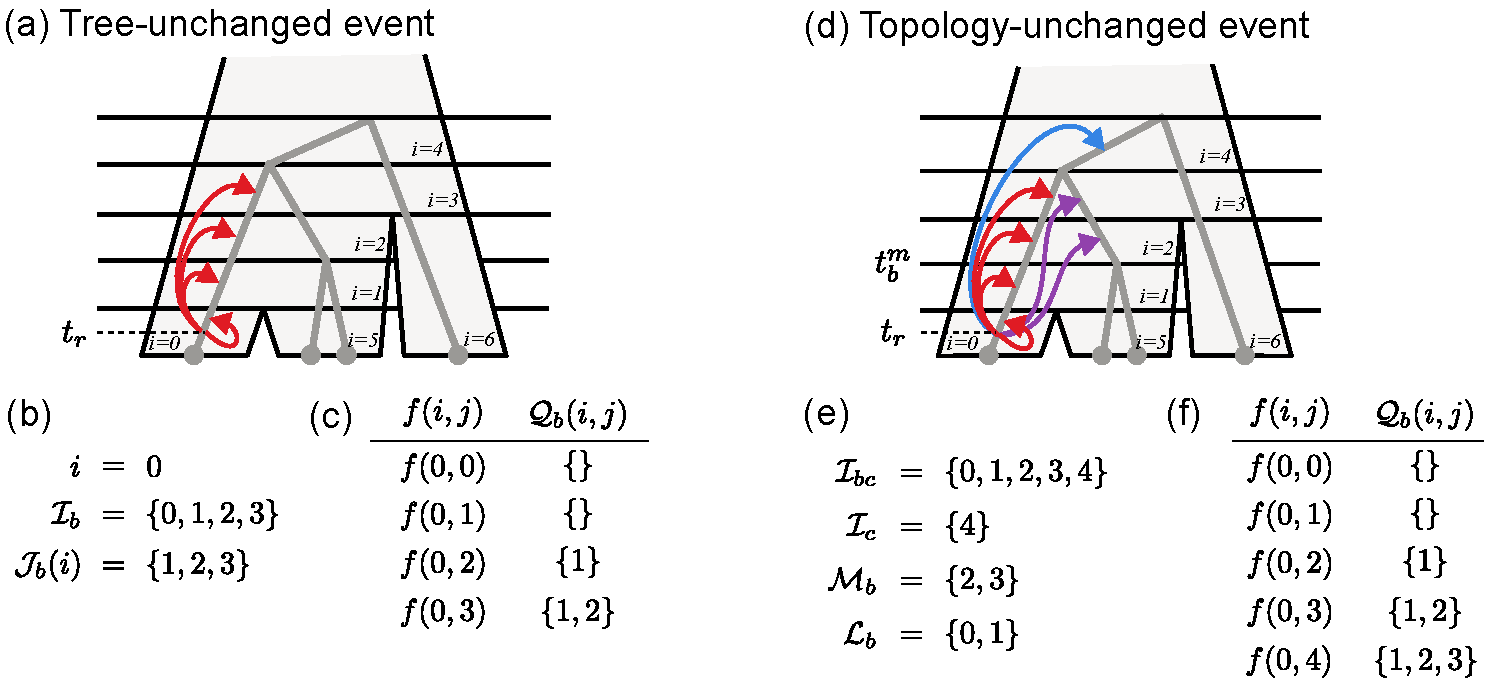
\includegraphics[width=0.99\textwidth]{figures/current/Fig3-interval-functions.pdf}
	\caption{
		The probability of each categorical
		recombination event type is calculated from the probability
		of recombination occurring on a specific gene tree branch and of
		the resulting detached subtree re-coalescing with an available
		branch above that event.
		(a) The probability of a ``no-change" (tree-unchanged) event involves
		re-coalescing with the same branch on which recombination occurred,
		for which intervals are indexed using the variable $\mathcal{I}_b$.
		(b) Indexing variables for calculating 
		no-change probabilities. The indexing variable $\mathcal{I}_b$ records all
		intervals on branch $b$; the recombination event for this example 
		occurs in interval $i$=0.
		$\mathcal{J}_b(i)$ returns all intervals in $\mathcal{I}_b$ above interval $i$.
		(c,f) The function $f(i,j)$ returns the probability that a subtree that detached 
		in interval $i$ will re-coalesce in interval $j$. This involves excluding
		the probability of re-coalescence in intervals between $i$ and $j$, which are 
		indexed as $\mathcal{Q}_b(i,j)$. 
		(d) The probability of a topology-unchanged event involves re-coalescing with the 
		same branch on which recombination occurred, or with its parent or sibling branches. 
		(e) Additional indexing variables return intervals on the parent branch 
		($\mathcal{I}_c$), or branch $b$ above ($\mathcal{M}_b$) or below 
		($\mathcal{L}_b$) the time ($t_b^m$) at which it overlaps in the same species tree interval 
		as its sibling branch.
	}
	\label{fig:fig3}
\end{figure}


% PREVIOUS APPROVED EQUATION 3
\begin{equation}
\begin{aligned}
	&\mathbb{P}(\text{no-change} | \mathcal{S},\mathcal{G},b,t_r) = 
	\frac{1}{k_i} + 
	f(i,i) \exp \bigg\{ \frac{k_i}{2n_i} t_r \bigg\} +
	\sum_{j \in \mathcal{J}_b(i)} f(i,j) \exp \bigg\{ \frac{k_i}{2n_i} t_r\bigg\}
\end{aligned}
\end{equation}


\noindent This equation is simplified by use of the function $f(i,j)$
to return the piece-wise constant probabilities of re-coalescence between
pairs of intervals. When $j$=$i$, this expression involves the probability of 
coalescing over the remaining length of interval $i$ above $t_r$; 
when $j$>$i$ it involves the probability of coalescing in interval 
$j$ and not coalescing in interval $i$ or any other intervals 
between $i$ and $j$. For this latter process, we define another
indexing variable, $\mathcal{Q}_b(i,j)$ = $\{q \in \mathcal{I}_b ~|~ j > q > i\}$, 
for iterating over the ordered intervals above $i$ and below $j$ 
on branch $b$ (e.g., Fig.~\ref{fig:fig3}c).
The function $f(i,j)$ forms the core of the MS-SMC algorithm and 
will reappear in several later equations. 
For didactic purposes, a step-by-step demonstration of equation (3) 
is shown in Fig.~\ref{fig:figS-tree-equations} of the Appendix.

\begin{equation}
\begin{aligned}	
	f(i,j) = 
	\begin{dcases}
		- \frac{1}{k_i} \exp \bigg\{-\frac{k_i}{2n_i}\mu_i \bigg\}, 
		& \text{if } i=j\\
		% 
		\frac{1}{k_j} \left(1 - \exp \bigg\{ -\frac{k_j}{2n_j} d_j \bigg\} 
		\right)
		\exp \bigg\{ -\frac{k_i}{2n_i}\mu_i - 
		\sum_{q \in \mathcal{Q}_b(i,j)} \frac{k_q}{2n_q} d_q \bigg \}, 
		& \text{if } i<j\\
		% 
		0, 
		& \text{if } i>j\\
	\end{dcases}
\end{aligned}
\end{equation}


\noindent By integrating equation 3 across all times at which recombination could
have occurred on branch $b$ (assuming a uniform recombination rate through time) 
we obtain the probability that recombination anywhere on this branch does not 
change the tree:


\begin{equation}
\begin{aligned}
	\mathbb{P}(\textrm{no-change} | \mathcal{S},\mathcal{G},b) = 
	\frac{1}{t_b^u - t_b^l}
	\sum_{i \in \mathcal{I}_b} \left[\frac{1}{k_i} d_i + 
	\frac{2n_i}{k_i} 
	\sum_{j \in \mathcal{I}_b}f(i,j)
	\bigg(
		\exp\bigg\{\frac{k_i}{2n_i}\mu_i \bigg\} - 
		\exp\bigg\{\frac{k_i}{2n_i}\sigma_i \bigg\}
	\bigg)\right]
\end{aligned}
\end{equation}


\noindent Finally, by summing across all branches on the tree 
while weighting each one by its relative proportion of edge length,
we get the probability that a recombination event occurring anywhere on 
$\mathcal{G}$ will result in a no-change event.

\begin{equation}
	\mathbb{P}(\text{no-change} | \mathcal{S},\mathcal{G}) = 
	\sum_{b \in \mathcal{G}}
	\left[\frac{t^u_b - t^l_b}{L(\mathcal{G})}\right]
	\mathbb{P}(\text{no-change} | \mathcal{S},\mathcal{G},b)
\end{equation}


\subsubsection{Waiting distances to no-change and tree-change events}
Under the SMC', recombination is modeled as a Poisson point process 
such that the time between recombination events is exponentially distributed 
with rate parameter $\lambda_r$: the product of the per-site
per-generation recombination rate and summed branch lengths of
the current genealogy \citep{wiuf_ancestry_1999} (equation 7).
The likelihood of an observed distance ($x$) between recombination
events spatially along the genome, in units of base pairs, can thus 
be calculated from the exponential probability density function 
(equation 8).

\begin{equation}
	\lambda_{r} = L(\mathcal{G}) \times r
\end{equation}

\begin{equation}
	f(x; \lambda_r) = \lambda_r e^{-\lambda_r x}
\end{equation}

\noindent Having derived the probability that an individual recombination event 
is of the no-change type, we can now calculate 
the rate of no-change type events as a proportion of the rate of all types of 
recombination events. 
Here, waiting distances continue to be exponentially distributed. 
However, the new rate parameter $\lambda_n$ is reduced proportionally by 
the probability that recombination causes no change to the genealogy
(equation 9). Similarly, because a tree-change event is the opposite 
of a no-change event, its probability is one minus the probability
of no-change (equation 10). This yields rate parameter $\lambda_g$ for 
the exponential probability distribution of waiting distances between 
tree-change events.

\begin{equation}
	\lambda_{n} = 
	L(\mathcal{G}) \times r \times 
	\mathbb{P}(\text{no-change} | \mathcal{S},\mathcal{G})
\end{equation}

\begin{equation}
	\lambda_{g} = 
	L(\mathcal{G}) \times r \times 
	(1 - \mathbb{P}(\text{no-change} | \mathcal{S},\mathcal{G}))
\end{equation}


\subsubsection{Probability of topology-change}
We next derive an analogous probability distribution for waiting distances 
between topology-change events.
Similar to our approach for calculating tree-change probabilities as the opposite of those for a 
no-change (tree-unchanged) event, here we calculate topology-change probabilities as the 
opposite of those for a topology-unchanged event. Topology-unchanged events represent the union of 
all no-change events and the subset of possible tree-change events 
that only affect branch lengths but not the topology. 
Our approach for calculating these probabilities follows closely to that of
\citet{deng_distribution_2021}.
In order to isolate re-coalescence events that do not change the topology,
we must take into account which specific branches the detached subtree from 
branch $b$ re-coalesces with. The relevant branches are its source ($b$), 
its sibling ($b'$), and its parent ($c$) (Fig.~\ref{fig:fig3}d). 
If the subtree re-coalesces with $b$, no change occurs; if it re-coalesces
with $b'$, the topology remains the same but a coalescent time is shortened;
and if it re-coalesces with $c$, the topology remains the same but a coalescent 
time is lengthened. A re-coalescence with any other branch will change the topology.

To index over relevant intervals across the three branches on which re-coalescence
can occur, we define several additional variables. The lowest time point in which both 
$b$ and $b'$ are present and exist within the same species tree interval is labeled 
$t_b^m$. For a branch $b$ with intervals $\mathcal{I}_b$, the subset of intervals 
below $t_b^m$ is $\mathcal{L}_b$, and the subset above is $\mathcal{M}_b$. 
The union of the sets of intervals on branches $b$ and $c$ is $\mathcal{I}_{bc}$
(Fig.~\ref{fig:fig3}e).

Once again, we begin by assuming knowledge of the branch on which a 
recombination event occurs and of that event's timing. This problem can be broken 
into two distinct cases: when $t_r$ occurs below $t_b^m$, and when it 
occurs above $t_b^m$. The former requires integrating over additional 
intervals on $b$ that are not shared with $b'$. Over all intervals
on the three relevant branches, these equations use the function 
$f(i,j)$ to return the piecewise constant probabilities where recombination 
occurs in interval $i$ and re-coalesces in interval $j$ (Fig.~\ref{fig:fig3}f).
We provide a didactic example of the Equation 11 calculation 
in Fig.~\ref{fig:figS-topo-equations} of the Appendix.

\begin{equation}
\begin{aligned}
	&\mathbb{P}(\textrm{topology-unchanged} | \mathcal{S},\mathcal{G},b,t_r)=
	\\
	&\begin{dcases}
		\frac{1}{k_i} + 
		\sum_{j \in \mathcal{I}_{bc}} f(i,j) \exp \bigg\{ \frac{k_i}{2n_i}t_r \bigg\} + 
		\sum_{j \in \mathcal{M}_b} f(i,j) \exp \bigg\{ \frac{k_i}{2n_i}t_r \bigg\}, 
		& \text{if } t_r < t_b^m \\
		\\
		2\bigg(
			\frac{1}{k_i} + 
			\sum_{j \in \mathcal{I}_b} f(i,j) \exp \bigg\{ \frac{k_i}{2n_i}t_r \bigg\}
		\bigg) + 
		\sum_{j \in \mathcal{I}_c} f(i,j) \exp\bigg\{ \frac{k_i}{2n_i}t_r \bigg\},
		& \text{if } t_r \ge t_b^m \\
	\end{dcases}
\end{aligned}
\end{equation}


\noindent Next, the probability of a topology-unchanged event given recombination 
anywhere on a branch can be derived by integrating the previous equation 
over the entire length of a branch.
Here, the terms $p_{b,1}$ and $p_{b,2}$ correspond to recombination occurring
on branch $b$ during a time that falls into either of the two cases in equation 11.

\begin{equation}
\begin{aligned}
	&\mathbb{P}(\textrm{topology-unchanged} | \mathcal{S},\mathcal{G},b) = 
	\frac{1}{t_b^u - t_b^l} \Bigg[
		\sum_{i \in \mathcal{L}_b} p_{b,1}^{(i)} + 
		\sum_{i \in \mathcal{M}_b} p_{b,2}^{(i)}
	\Bigg]
	\\
	&~~where: 
	\\
	&p_{b,1}^{(i)} = 
		\frac{1}{k_i} \Bigg[
			d_i + 2n_i \Bigg(
				\exp\bigg\{ \frac{k_i}{2n_i}\mu_i \bigg\} - 
				\exp\bigg\{ \frac{k_i}{2n_i}\sigma_i\bigg\}
			\Bigg)
		\Bigg(
			\sum_{j \in \mathcal{I}_{bc}}f(i,j) + \sum_{j \in \mathcal{M}_b}f(i,j)
		\Bigg)
	\Bigg]
	\\
	&~~and: 
	\\
	&p_{b,2}^{(i)} = 
		\frac{1}{k_i} \Bigg[
			2d_i + 2n_i \Bigg(
				\exp\bigg\{\frac{k_i}{2n_i}\mu_i \bigg\} - 
				\exp\bigg\{\frac{k_i}{2n_i}\sigma_{i} \bigg\}
			\Bigg)
		\Bigg(
			2\sum_{j \in \mathcal{I}_b} f(i,j) + \sum_{j \in \mathcal{I}_c} f(i,j)
		\Bigg)
	\Bigg]
    \end{aligned}
\end{equation}

\noindent Finally, by summing equation 12 across all branches on a 
genealogy while weighting each by its proportion of summed branch lengths,
we get the probability that a recombination event falling 
uniformly on the genealogy will result in a topology-unchanged event.

\begin{equation}
\begin{aligned}
	&\mathbb{P}(\textrm{topology-unchanged} | \mathcal{S},\mathcal{G})
	= \sum_{b \in \mathcal{G}}\frac{t_b^u - t_b^l}{L(\mathcal{G})} 
	\times 
	\mathbb{P}(\textrm{topology-unchanged} | \mathcal{S},\mathcal{G},b)
	\\
	&
	= \frac{1}{L(\mathcal{G})} \sum_{b \in \mathcal{G}}
	\bigg[ 
		\sum_{i \in \mathcal{L}_b} p_{b,1}^{(i)} +
		\sum_{i \in \mathcal{M}_b} p_{b,2}^{(i)}
	\bigg]
\end{aligned}
\end{equation}

\subsubsection{Waiting distance to topology-change events}
A recombination event either does or does not change the topology
of a genealogy, and we can therefore get the probability of a 
topology-change event using our topology-unchanged probability statement.
As with the previous waiting distance distributions, the distance between
topology-change events given a parameterized MSC model can be 
modeled as an exponential probability distribution. 
Similar to how a rate parameter was derived for the distribution 
of waiting distances until a recombination event (equation 7), 
no-change event (equation 9), or tree-change event (equation 10), 
a rate parameter $\lambda_t$ can be calculated from equation 13 for 
the probability of a topology-change event. 

\begin{equation}
	\lambda_{t} = 
	L(\mathcal{G}) \times r \times 
	(1 - \mathbb{P}(\text{topology-unchanged} | \mathcal{S},\mathcal{G}))
\end{equation}


Unlike the exact solution for the expected waiting distance to a  
tree-change, the waiting distance for a topology-change is an
approximation. This is because topology-change probabilities are not 
guaranteed to be homogeneous across some distance of the genome between 
topology-change events, since intermediate tree-change events could occur
(e.g., the second and third recombination events in Fig.~\ref{fig:ARG-cartoon}).
We examine this and other potential sources of bias in our validations
below and in the Supplementary Materials.


%%%%%%%%%%%%%%%%%%%%%%%%%%%%%%%%%%%%%%%%%%%%%%%%%%%%%%%%%%%%%%%%%%%%%%%%%%%
%%%%%%%%%%%%%%%%%%%%%%%%%%%%%%%%%%%%%%%%%%%%%%%%%%%%%%%%%%%%%%%%%%%%%%%%%%%
%%%%%%%%%%%%%%%%%%%%%%%%%%%%%%%%%%%%%%%%%%%%%%%%%%%%%%%%%%%%%%%%%%%%%%%%%%%
%%%%%%%%%%%%%%%%%%%%%%%%%%%%%%%%%%%%%%%%%%%%%%%%%%%%%%%%%%%%%%%%%%%%%%%%%%%
%%%%%%%%%%%%%%%%%%%%%%%%%%%%%%%%%%%%%%%%%%%%%%%%%%%%%%%%%%%%%%%%%%%%%%%%%%%
%%%%%%%%%%%%%%%%%%%%%%%%%%%%%%%%%%%%%%%%%%%%%%%%%%%%%%%%%%%%%%%%%%%%%%%%%%%
%%%%%%%%%%%%%%%%%%%%%%%%%%%%%%%%%%%%%%%%%%%%%%%%%%%%%%%%%%%%%%%%%%%%%%%%%%%
%%%%%%%%%%%%%%%%%%%%%%%%%%%%%%%%%%%%%%%%%%%%%%%%%%%%%%%%%%%%%%%%%%%%%%%%%%%
%%%%%%%%%%%%%%%%%%%%%%%%%%%%%%%%%%%%%%%%%%%%%%%%%%%%%%%%%%%%%%%%%%%%%%%%%%%
%%%%%%%%%%%%%%%%%%%%%%%%%%%%%%%%%%%%%%%%%%%%%%%%%%%%%%%%%%%%%%%%%%%%%%%%%%%
%%%%%%%%%%%%%%%%%%%%%%%%%%%%%%%%%%%%%%%%%%%%%%%%%%%%%%%%%%%%%%%%%%%%%%%%%%%
%%%%%%%%%%%%%%%%%%%%%%%%%%%%%%%%%%%%%%%%%%%%%%%%%%%%%%%%%%%%%%%%%%%%%%%%%%%
%%%%%%%%%%%%%%%%%%%%%%%%%%%%%%%%%%%%%%%%%%%%%%%%%%%%%%%%%%%%%%%%%%%%%%%%%%%
%%%%%%%%%%%%%%%%%%%%%%%%%%%%%%%%%%%%%%%%%%%%%%%%%%%%%%%%%%%%%%%%%%%%%%%%%%%
%%%%%%%%%%%%%%%%%%%%%%%%%%%%%%%%%%%%%%%%%%%%%%%%%%%%%%%%%%%%%%%%%%%%%%%%%%%
%%%%%%%%%%%%%%%%%%%%%%%%%%%%%%%%%%%%%%%%%%%%%%%%%%%%%%%%%%%%%%%%%%%%%%%%%%%
%%%%%%%%%%%%%%%%%%%%%%%%%%%%%%%%%%%%%%%%%%%%%%%%%%%%%%%%%%%%%%%%%%%%%%%%%%%
%%%%%%%%%%%%%%%%%%%%%%%%%%%%%%%%%%%%%%%%%%%%%%%%%%%%%%%%%%%%%%%%%%%%%%%%%%%
%%%%%%%%%%%%%%%%%%%%%%%%%%%%%%%%%%%%%%%%%%%%%%%%%%%%%%%%%%%%%%%%%%%%%%%%%%%
%%%%%%%%%%%%%%%%%%%%%%%%%%%%%%%%%%%%%%%%%%%%%%%%%%%%%%%%%%%%%%%%%%%%%%%%%%%


\section{Results}

\subsection{Implementation}
We have implemented our solutions for waiting distance calculations
under the MS-SMC in the Python package \emph{ipcoal} \citep{mckenzie_ipcoal_2020}.
This software includes functions that accept a parameterized MSC model and 
initial genealogy as input and return the probabilities of different 
recombination event types. These probabilities can be calculated for specific 
branches and times, for entire branches, or for entire genealogies. 
Functions are also available to calculate the expected waiting distances 
for a genealogy embedded in an MSC model,
and the likelihood of MSC model parameters given a distribution 
of waiting distances between tree-change or topology-change events in an ARG.
Our implementation is built upon \emph{toytree} \citep{eaton_toytree_2020}, 
\emph{scipy} \citep{2020SciPy-NMeth}, and 
\emph{numpy} \citep{harris2020array}, and 
uses jit-compilation with \emph{numba} 
\citep{lam2015numba}.
Below we use \emph{ipcoal} v.0.5.0 to demonstrate the impact of 
MSC model parameters on waiting distances and to validate our solutions against 
expectations from coalescent simulations implemented in 
\emph{msprime} (v.1.1.1) \citep{baumdicker_efficient_2022}.
Source code is available at \url{https://github.com/eaton-lab/ipcoal}.
Jupyter notebooks demonstrating the MS-SMC calculations and with 
reproducible code used for validations in this study are available
at \url{https://github.com/eaton-lab/waiting-distance-code}.


\begin{figure}
	\centering
	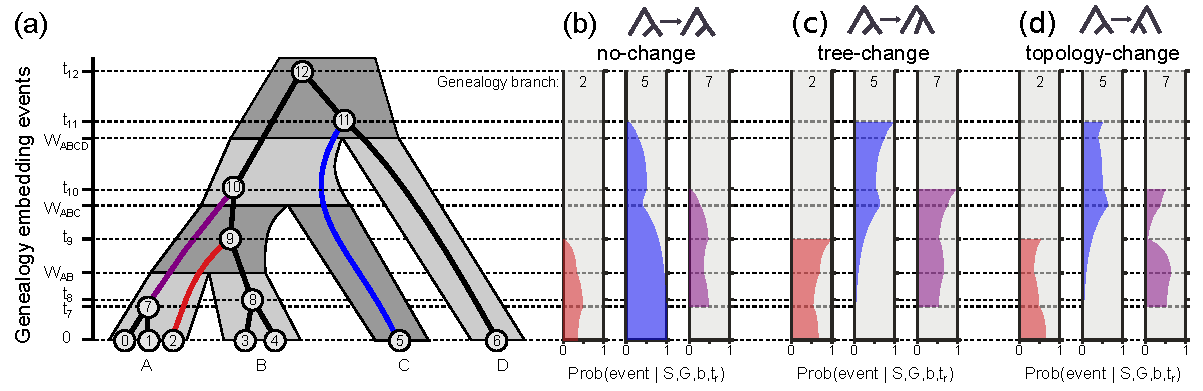
\includegraphics[width=0.99\textwidth]{figures/current/Fig4-embedding-with-probabilities.pdf}
	\caption{
		The MS-SMC is a model of the probability of different categorical event
		outcomes given recombination occurring uniformly on a genealogy embedded
		in a parameterized MSC model (a). 
		A recombination event can cause one of three possible recombination 
		event types between two sequential genealogies in a genome: 
		\emph{no-change}, \emph{tree-change}, or \emph{topology-change}.
		The probability of these event types are calculated by integrating over
		each branch on the genealogy on which recombination can occur; which
		in turn is calculated by integrating over each position on a genealogy
		branch at which recombination can occur.
		(b-d) The probability that a recombination event causes a no-change, tree-change, or topology-change event, for the example genealogy 
		embedded in a species tree, was calculated for three selected 
		genealogy branches (2: red; 5: blue; and 7: purple), at each position
		along the branch where recombination could occur.
	}
	\label{fig:edge-probabilities}
\end{figure}


\subsection{Demonstration}
Given a parameterized MSC model and initial genealogy, the probabilities of 
different types of recombination outcomes can be calculated and visualized as 
a function of when and where recombination occurs. This is demonstrated on an 
imbalanced 4-tip species tree with constant effective population size 
and with a genealogy of seven samples embedded, 
including three from lineage A, two from lineage B, and one from each of lineages
C and D (Fig.~\ref{fig:edge-probabilities}a). 
(See Fig.~\ref{fig:figS-edge-probabilities} for details and
alternative parameterizations of this simulation.)
The probabilities of no-change, tree-change, or topology-change events, 
given a recombination event occurring on a branch at a particular time 
(equations 3 and 11, respectively) are shown for three selected branches
on the example genealogy (Fig.~\ref{fig:edge-probabilities}b-d). 
Note that the probability of no-change and tree-change events 
are inversely related and sum to 1, since one or the other must occur at any 
recombination event. By contrast, the probability of a 
topology-change event is a subset of the probability of a tree-change 
event;
it is a tree-change event where the detached branch re-coalesces with 
a branch other than itself, its sibling, or its parent.


In general, the probability of a no-change event decreases, and the probability
of a tree-change event increases, as recombination occurs closer to the top
of a genealogy branch (further back in time). 
This makes intuitive sense, since when 
recombination occurs at the top of a branch there is less time for it to re-coalesce 
with its same branch. Although this is a general trend, these probabilities do not 
behave monotonically with respect to time as they would in a 
single-population model with constant $N_e$ \citep{deng_distribution_2021}.
Instead, probabilities increase or decrease through the length of each
interval as a function of the rates of coalescence in subsequent 
intervals and the probability that a detached lineage will 
re-coalesce in one of those intervals.

For example, consider genealogy branch 2, which exhibits an increase in the
probability of no-change through its first branch interval from time 0 to
$t_7$ but then a decrease through the next interval from $t_7$ to $W_{AB}$
(Fig.~\ref{fig:edge-probabilities}b).
The observed increase through the first interval is influenced by the fact that
a re-coalescence in the subsequent interval is more likely to cause a no-change
event, since that interval contains only two samples instead of three.
By contrast, within the second interval, recombination events near 
the top are approaching the next species tree divergence event. After that event, the 
number of samples will increase back from 2 to 3, 
thus decreasing the probability of a no-change event. 
This visualization demonstrates how the probabilities of different recombination 
event types represent an integration over all the positions on a branch where 
recombination could occur, and all positions at or above each of these points (whether on the 
same or different available branches) where a detached subtree could re-coalesce. 

Genealogy branch 7 provides a clear example for examining the probabilities of 
tree- and topology-change events. Of particular interest is the 
interval from $W_{AB}$ to $W_{ABC}$ where these probabilities diverge 
significantly (Fig.~\ref{fig:edge-probabilities}c-d). 
The probability of topology-change decreases faster than the probability of 
tree-change as recombination occurs closer to node $t_9$. This is because 
following $t_9$ there is a large stretch of time during which re-coalescence can
only occur with the same branch or its sibling, neither of which can cause a topology-change
event. It is only after $W_{ABC}$ that it is once again possible for re-coalescence
to occur with a more distant branch that would result in topology-change. 
If the effective population size of this species tree interval (AB) were greater,
then the probability of re-coalescence in a deeper interval would be more likely, 
and the probability of topology-change would decrease less severely near $t_9$. 
This is true more generally, as can be seen by comparing edge probabilities
across MSC models with different effective population sizes (Fig.~\ref{fig:figS-edge-probabilities}).
Effective population size affects the rate of re-coalescence and thus 
either smooths probabilities across intervals when 
$N_e$ is high or accentuates differences among intervals when $N_e$ is low.


\subsection{Validation}

\begin{figure}[tp]
	\centering
	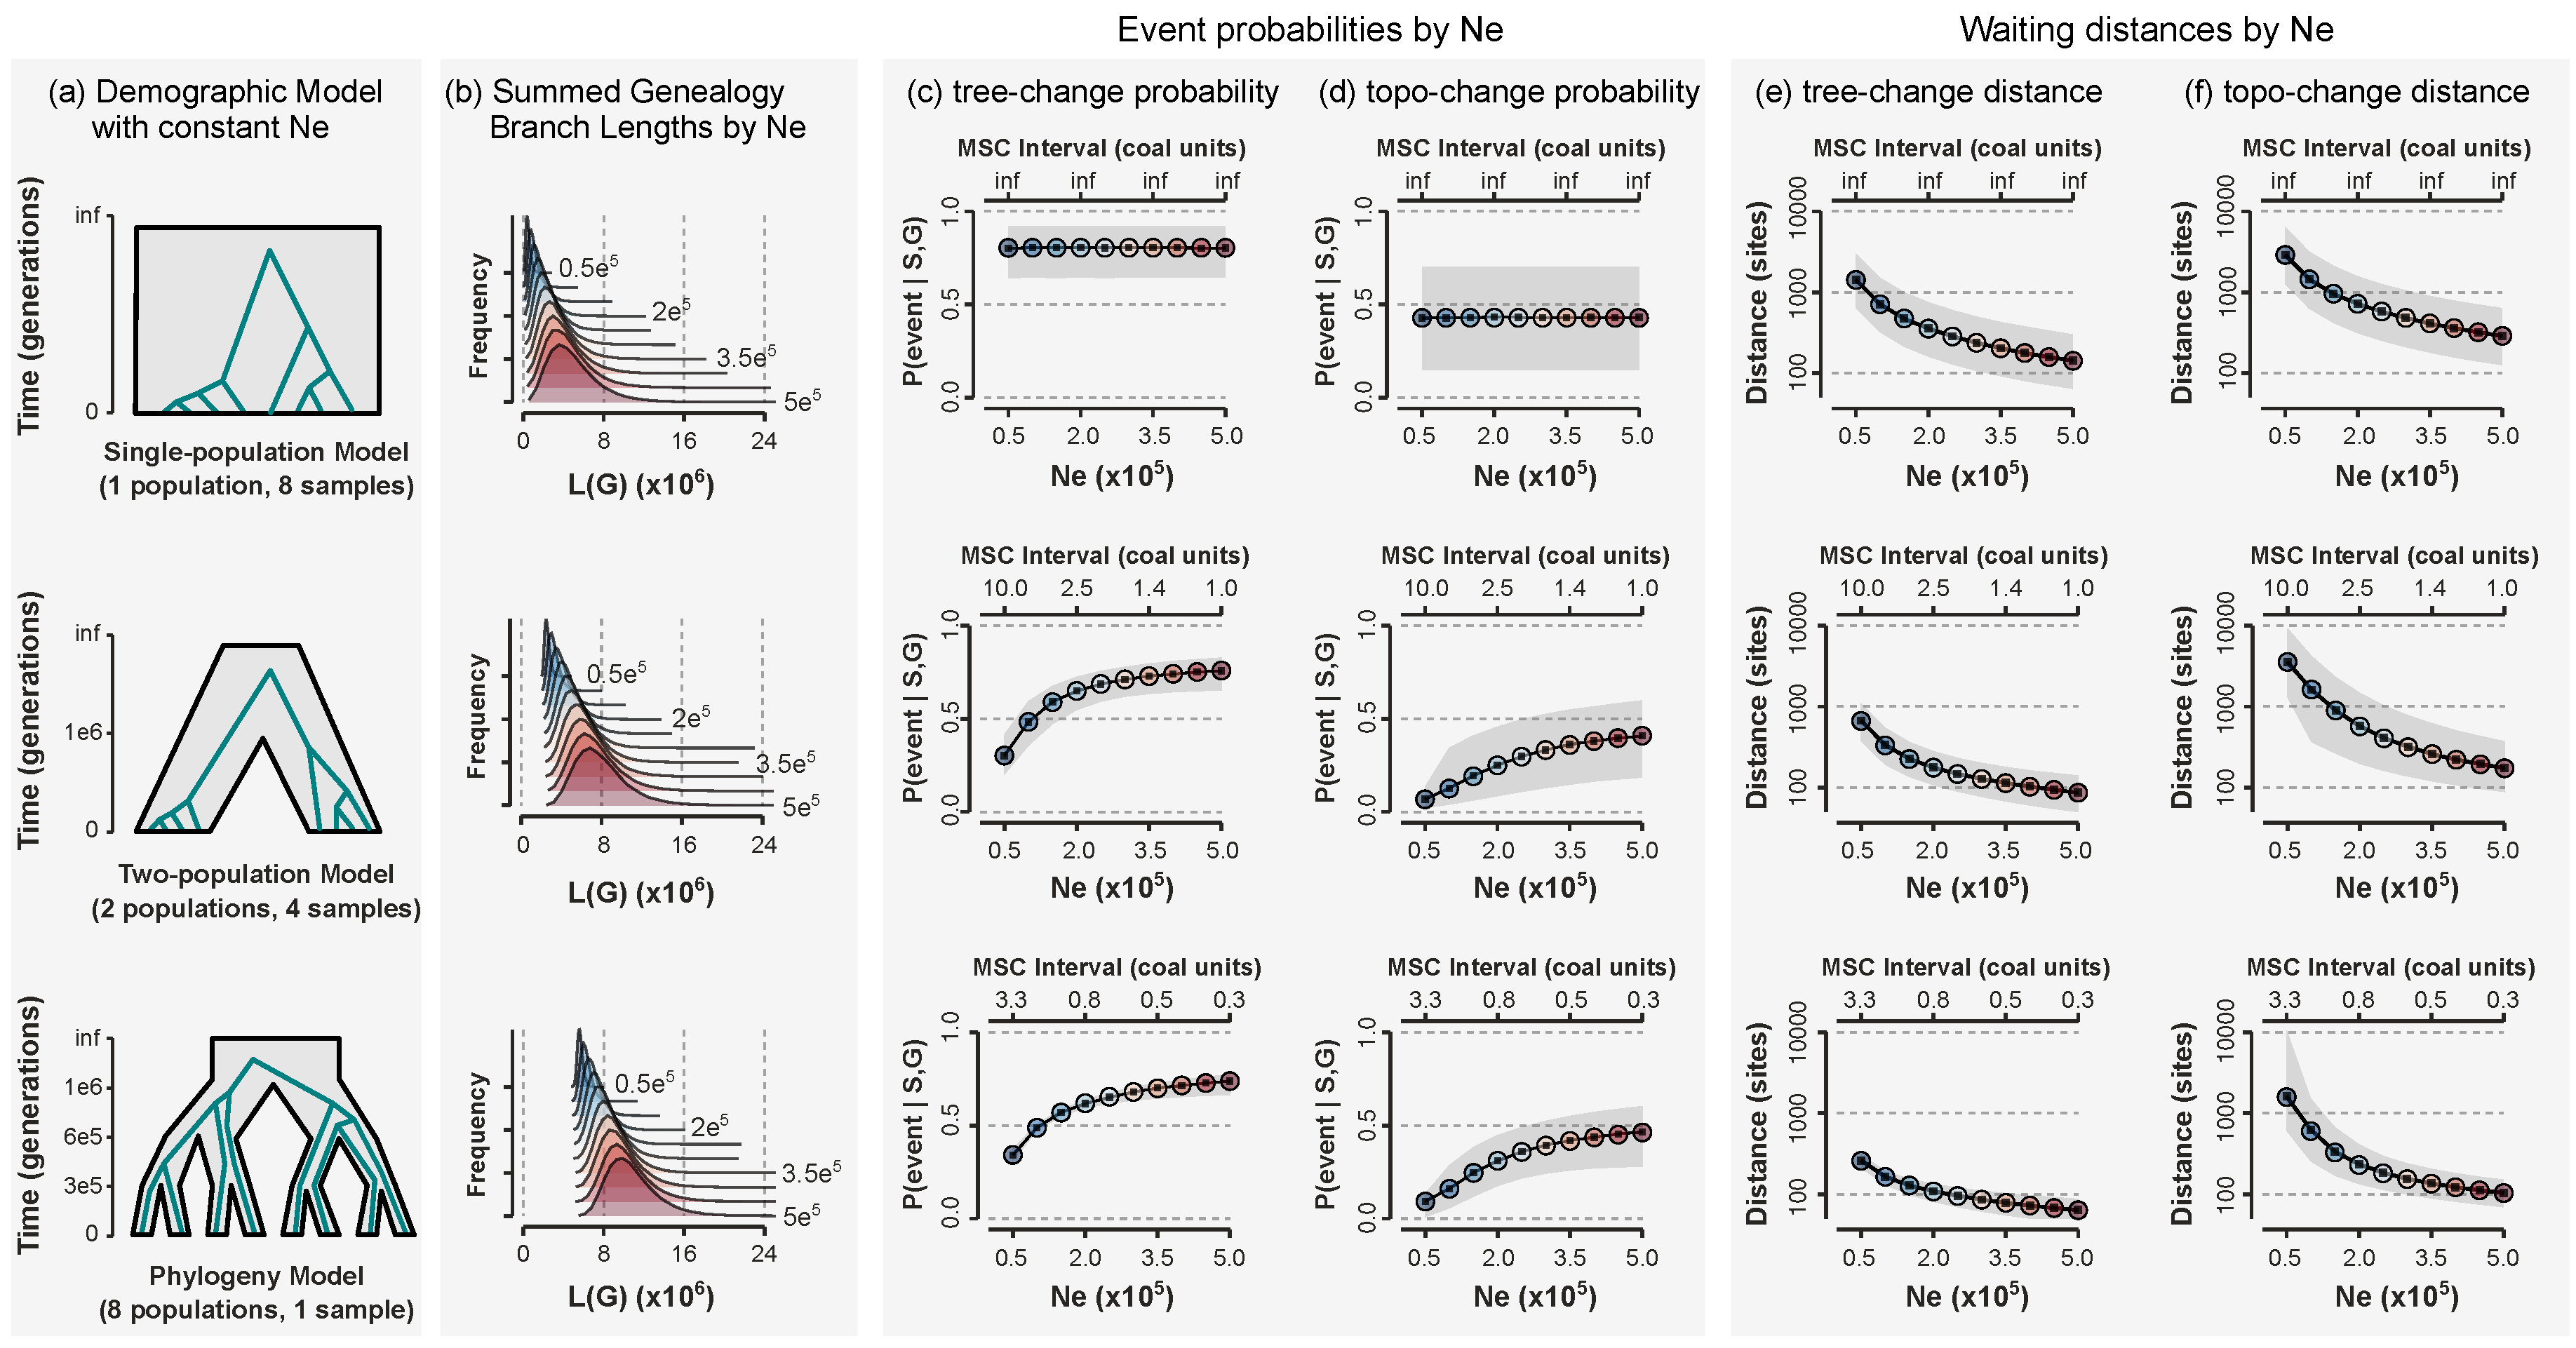
\includegraphics[width=0.99\textwidth]{figures/current/Fig5-validation-sims-NEW4.pdf}
	\caption{
		MS-SMC predictions validated against coalescent simulations.
		(a) Results are shown for three models containing 1, 2, or 8 
		populations. 
		For each model, 100K tree sequences were simulated for 10 different
		constant $N_e$ values between 50K and 500K. 
		(b) The distributions of summed edge lengths of the first genealogy in 
		each tree sequence. 
		(c-d) The mean frequency (black square) with which the first observed 
		recombination event was a tree-change (c) or topology-change (d) in a 
		simulated tree sequence, and the mean (colored circle) and 95\% CI 
		(grey fill) of the predicted probability of tree or topology-change 
		calculated from the first embedded genealogy in each tree sequence. 
		Probabilities are constant with respect to $N_e$ in the single population
		model but vary in models with population structure
		(also shown with respect to species tree interval lengths in 
		coalescent units, across the top axis).
		(e-f) The mean waiting distance (black square) until the first observed 
		tree-change (e) or topology-change (f) in a simulated tree sequence, and the mean 
		(colored circle) and 95\% CI (grey fill) of predicted waiting distances calculated
		using the first embedded genealogy in each tree sequence.
	}
	\label{fig:fig-validation}
\end{figure}


To validate our analytical solutions for the probabilities of different 
recombination event outcomes and their associated waiting distances, 
we compared predictions of the MS-SMC with results from stochastic 
coalescent simulations. 
We set up three scenarios with increasing amounts of population structure: 
a single-population model, a two-population model, and an 8-tip phylogeny model
(Fig.~\ref{fig:fig-validation}a). 
All analyses used a constant per-site per-generation recombination rate of 
2e-9 and simulated tree sequences using the coalescent with recombination 
(i.e., the "hudson" ancestry model in msprime as opposed to the "smc\_prime" model, 
which is an approximation),
and the argument 
"record\_full\_arg=True" (to retain records of invisible recombination events). 
For each model we simulated genealogies for the same total number of samples
(8, unless specified), divided evenly among lineages when models 
include multiple populations (Fig.~\ref{fig:fig-validation}a). 


The exponential rate parameter ($\lambda$) for a probability distribution of waiting distances 
is a product of the per-site per-generation recombination rate ($r$), the sum 
of edge lengths on the current genealogy ($L(\mathcal{G})$), and the probability 
($\mathbb{P}$) of the specified event type (equations 9, 10, and 14). 
Across the three models examined, $r$ remains constant, but both $L(\mathcal{G})$ 
and $\mathbb{P}$ can vary due to population structure, where the effect of 
structure is scaled by $N_e$. 
Therefore, we examined $L(\mathcal{G})$, $\mathbb{P}$, and the expected waiting 
distance calculated from their product, for each demographic model across a range 
of $N_e$ values (50K -- 500K; Fig.~\ref{fig:fig-validation}b-f). 
At each value of $N_e$ we simulated 100K tree sequences for each
demographic model.

Each simulated tree sequence
contains a series of trees and intervals representing stochastic outcomes of
the coalescent with recombination. Over many replicates, we expect the mean
waiting distances until the first tree and topology-change events in simulations 
to match the predicted waiting distances estimated under the MS-SMC, computed
from only observing the starting tree in each tree sequence.
(Note that to avoid any potential bias associated with the first tree interval 
in simulated tree sequences we actually advanced to the first tree after the 
first topology-change event to serve as the starting tree in all analyses.) 
To measure tree and topology-change waiting distances in tree sequences we 
recorded the sum length of the interval that includes the starting tree, and any 
subsequent intervals in which no tree-change occurred, or no topology-change 
occurred, respectively. To measure the probability of each event type in simulations
we recorded which event type (including no-change events) was the first to occur 
after the starting tree in each tree sequence. 
The MS-SMC probabilities of each event type were computed in \emph{ipcoal} by 
embedding the starting tree of each tree sequence into the parameterized MSC model.
Expected waiting distances under the MS-SMC were computed as 1 over the product 
of the event probabilities, $r$, and $L(\mathcal{G})$ of the starting tree.

Population structure enforces a 
limit on the minimum length of coalescent 
times by requiring that genealogies can be embedded in a species tree.
This has the effect of shifting both the minimum and mean of 
$L(\mathcal{G})$ higher 
across all values of $N_e$ (Fig.~\ref{fig:fig-validation}b). 
Because the per-generation recombination rate interacts with
$L(\mathcal{G})$ (the opportunity over which recombination can occur) to
determine the frequency of recombination, larger $L(\mathcal{G})$ induced
by population structure will tend to decrease waiting distances between 
recombination events, all else being equal. 
However, all else does not remain equal.
Instead, population structure in MSC models has a simultaneous opposing effect
of increasing the mean waiting distance to tree or topology change events by 
affecting the event probabilities
(Fig.~\ref{fig:fig-validation}c-d).
This is most clear at low values of $N_e$, where shorter coalescent times are
less likely to span the barriers between lineages in an MSC model. 
This has the effect of increasing the probability of no-change events
relative to tree or topology-change events. By contrast, when $N_e$ is high the 
barriers in an MSC model have little effect on coalescence probabilities, and 
the tree and topology-change event probabilities in MSC models converge towards 
those seen in the single population model
(Fig.~\ref{fig:fig-validation}c-d). 
This highlights the relationship between MSC model parameters and the waiting 
distances between different recombination event types. In MSC models, waiting
distances to the three different recombination event types can vary as a 
consequence of the model parameters' effects on $L(\mathcal{G})$ and $\mathbb{P}$, 
whereas in a single population model each waiting distance is simply scaled 
by $L(\mathcal{G})$.


Our analytical predictions under the MS-SMC converge accurately on 
the mean results from stochastic coalescent simulations 
(Fig.~\ref{fig:fig-validation}c-f). 
Moreover, by examining the variance in these predictions with 
respect to MSC model parameters we further gain insights into 
the information contained in spatial genealogical patterns.
For example, in the single population model there is high variance 
in both the probabilities of tree and topology changes, as well as in genealogy
lengths, at any given $N_e$ value. Consequently, waiting distances also 
exhibit high variance. Although waiting distances correlate with population $N_e$ 
in this model, the differences in mean waiting distances are small relative to the variance. 
By contrast, multispecies models exhibit much less variance in predicted probabilities 
of tree or topology changes given a set of MSC model parameters 
(Fig.~\ref{fig:fig-validation}c-d) and also exhibit less variation in genealogy
lengths. This leads to a stronger relationship between MSC model parameters and 
expected waiting distances (Fig.~\ref{fig:fig-validation}e-f), such that models
with different parameters have less overlap in waiting distance expectations.
Overall, this demonstrates that estimations of tree- and topology-change
waiting distances calculated under the MS-SMC are accurate, and contain 
information for inferring population demographic parameters.

\subsection{Bias in waiting distance estimation}
Estimated waiting distances under the MS-SMC harbor two potential sources of bias, 
the first stemming from assumptions of the SMC' approximation, and the second from 
the approximate nature of waiting distance estimation for topology-change events. 
We examined both of these sources of error through comparison to stochastic simulations
and found that their effects are generally small, and that multispecies models exhibit 
a similar magnitude of error as single population coalescent models 
(see "Investigating bias" section in Supplementary Materials; 
Fig.~\ref{fig:figS-bias-smc}, 
Fig.~\ref{fig:figS-bias-topo-first}, 
Fig.~\ref{fig:figS-bias-topo-last}).
The SMC' approximation introduces very little bias to MS-SMC estimates of 
tree-change waiting distances across all scenarios examined, and only 
significantly biases topology-change waiting distance estimates in the 
"species tree" demographic model scenario at very low $N_e$ values -- a 
scenario where genealogical discordance becomes very unlikely. 
This scenario is also most affected by the other source of bias, as
it exhibits greatest variance in genealogy branch lengths among
intervals between topology-change events. For both sources of bias, 
we show that error is greatly reduced by simply increasing the number
of genomes sampled per lineage.


\subsection{A Likelihood-based Framework for Evaluating Waiting Distances}

The MS-SMC is a statistical model of the waiting distances between different
types of genealogy changes in an ARG, given a parameterized MSC model. 
Since waiting distances between recombination events follow an exponential 
distribution, we can use the exponential probability density (equation 8) 
as the likelihood function to assess observed (or estimated) waiting
distances in an ARG, by modeling the probability of these waiting distances
as a function of demographic model parameters.
We propose that applications of this approach can provide 
improvements to ARG and demographic model inference methods. Below, we
describe and demonstrate one such application.

Given one or more ARGs each composing a sequence of genealogies and
their interval lengths in a genome, 
a subset of genealogies and intervals can be extracted that represent 
the combined intervals between a specific type of event
(Fig.~\ref{fig:likelihood-calculation}a).
For example, $\boldsymbol{\mathcal{G}_g}$ = ($\mathcal{G}_1, \mathcal{G}_j, ...$)
can represent
the subset of genealogies that occur between tree-change events
and $\boldsymbol{X_g}$ = ($\sum_{i=1}^j x_i, \sum_{i=j}^{k} x_i, ..., $)
the summed lengths of intervals between tree-change events
(Fig.~\ref{fig:likelihood-calculation}b-c).
The same can be done for topology-change events.
Given a parameterized MSC model and recombination rate
we can then obtain a set of exponential rate parameters
$\boldsymbol{\Lambda_g} = (\lambda_1, \lambda_j, ...)$ for the waiting distance 
until the next tree-change for each genealogy in $\boldsymbol{\mathcal{G}_g}$ 
(equation 10; Fig.~\ref{fig:likelihood-calculation}d).
Finally, using the exponential probability density function,
the likelihood of the MSC model parameters is calculated as the
product of the probability densities for each waiting distance
in $\boldsymbol{X_g}$, evaluated using the corresponding rate parameters in 
$\boldsymbol{\Lambda_g}$
(Fig.~\ref{fig:likelihood-calculation}e).
Maximum likelihood optimization of the model parameters can be achieved
by identifying the set of parameters -- affecting $\boldsymbol{\Lambda_g}$ -- that
maximize the likelihood function, which quantifies the probability of 
the observed data given the model.


\begin{figure}[tp]
	\centering
	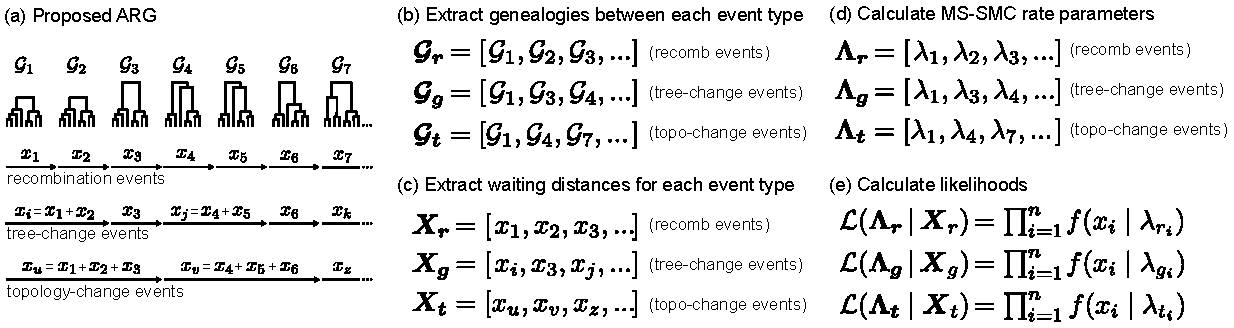
\includegraphics[width=0.99\textwidth]{figures/current/Fig6-ARG-likelihood-steps-full.pdf}
	\caption{
		A likelihood framework for fitting MSC model parameters from waiting distances
		between categorical types of recombination events in an ARG.
		(a) An ARG represents a sequence of genealogies ($\mathcal{G}$) and their
		interval lengths ($x$) over a genomic region. Intervals can be delimited 
		by all recombination events, or by a subset representing only tree-change, 
		or only topology-change events.
		(b) The set of genealogies ($\boldsymbol{\mathcal{G}}$) occurring between
		each event type can be extracted, and similarly, 
		(c) the set of associated interval lengths ($\boldsymbol{X}$) between
		each event type can be extracted.
		(d) A set of exponential rate parameters ($\boldsymbol{\Lambda}$) can 
		then be estimated under the MS-SMC for the waiting distance until 
		each type of recombination event, for each genealogy, given its 
		embedding in a parameterized MSC model
		($\mathcal{S}$) and the recombination rate ($r$).
		(e) Using the exponential probability density function, the likelihood 
		of the MSC model parameters is calculated as the product of the 
		probability densities for each waiting distance in $\boldsymbol{X}$,
		evaluated using the corresponding rate parameters in 
		$\boldsymbol{\Lambda}$.
	}
	\label{fig:likelihood-calculation}
\end{figure}


\begin{figure}[p]
	\centering
	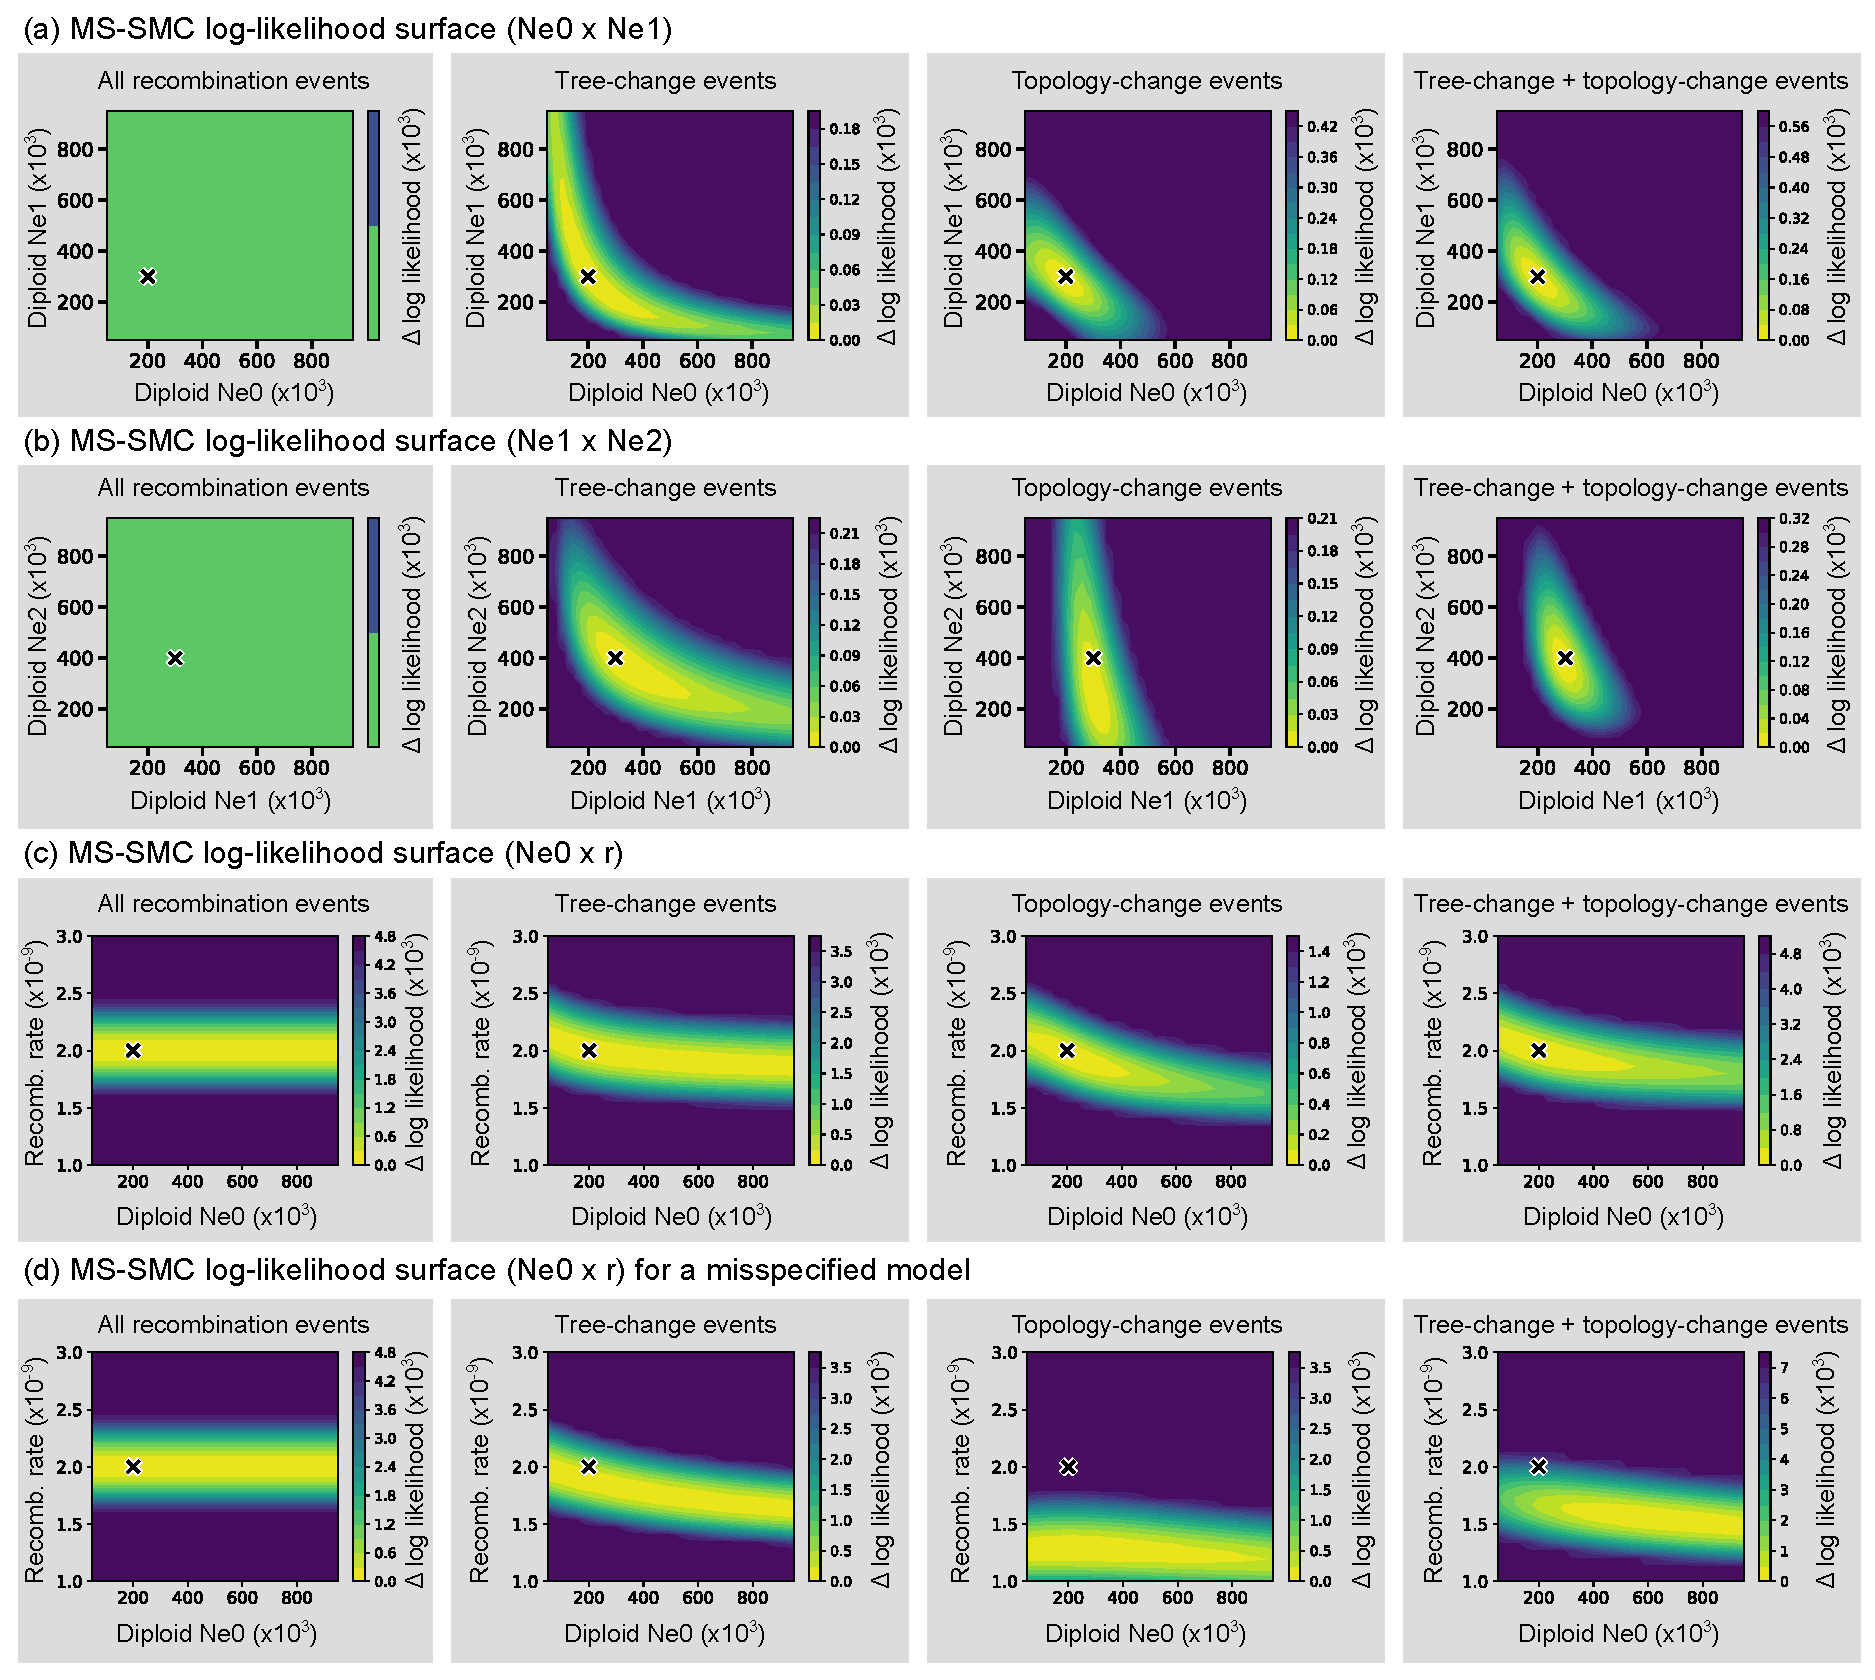
\includegraphics[width=0.99\textwidth]{figures/current/Fig7-likelihood-surfaces-MCMC3.pdf}
	\caption{
		Implementation of a likelihood framework for fitting MSC model parameters
		to waiting distances in an ARG. Tree sequences were simulated under a 
		2-population demographic model with four MSC parameters ($N_e$0=200K, 
		$N_e$1=300K, $N_e$2=400K, $W$=1M) and recombination rate $r$=2 x 10$^{-9}$. 
		Log-likelihood surfaces are shown for two parameters at a time while fixing
		other parameters to their true value. True values are marked by an X.
		(a-c) Waiting distances between all recombination events provide no information
		for estimating MSC parameters, but the waiting distances between tree-change 
		and topology-change events are informative about MSC parameters, both
		individually and in combination.
		(d) When waiting distances derived from a 2-population model are used to 
		fit parameters in a single-population model they provide poor estimates
		of MSC parameters.
	}
	\label{fig:likelihood-surfaces}
\end{figure}


We implemented this approach to evaluate MSC model parameters 
using waiting distances in an ARG simulated under a two-population MSC model with 
variable $N_e$ ($N_e$0=200K, $N_e$1=300K, and $N_e$2=400K), a divergence time
$W$=1M generations, and recombination rate $r$=2e-9. We sampled four 
genomes per population, and simulated 50 independent tree sequences 
each 400Kb in length (20Mb total) under the full coalescent with 
recombination model.
This yielded 235,872 intervals between recombination events
(mean +/- S.D. length = 84.79 +/- 92.90), composing 
160,501 intervals between tree-change events
(mean +/- S.D. length = 124.56 +/- 135.68),
and 59,288 intervals between topology-change events
(mean +/- S.D. length = 336.93 +/- 441.72).
To examine the information contained in different waiting distance data
sets we visualized 2D log-likelihood surfaces over a grid of 
values for pairs of MSC model parameters, while keeping all other 
parameters fixed at their true values.

We compared log-likelihood surfaces for four different sources of waiting
distance information, comprising the waiting distances between all 
recombination events, between only tree-change events, between only 
topology-change events, and for the combined log-likelihoods from both 
tree-change and topology-change waiting distances. 
(Fig.~\ref{fig:likelihood-calculation}e). 
Note that combining tree-change and topology-change likelihoods may seem 
like double-counting of information, since topology-change events are a
subset of the events that compose a tree-change event, in our terminology.
However, our equation for the probability of a topology-change event is 
conditional only on $\mathcal{S}$ and $\mathcal{G}$, and not on the probability 
of one or more tree-change events.
In addition, it is clear conceptually that these two types of event 
probabilities have different relationships with a species tree.
As an example, consider a genealogy that has two genomes sampled per species,
and is embedded in a species tree with very low $N_e$ such that ILS is nearly 
impossible. The probability of a topology-change event approaches zero
in this scenario, whereas the probability of a tree-change event is
much less affected by species tree barriers, since this event type can still 
occur within each species tree interval as a change in coalescent times.
We demonstrate below how the likelihood of a demographic model can be more
robustly assessed by jointly incorporating both types of waiting distance
observations into the likelihood calculation.


The log-likelihood surfaces show that waiting distance information
in an ARG is informative for estimating MSC model parameters when 
analyzed under our MS-SMC model framework
(Fig.~\ref{fig:likelihood-surfaces}). 
The waiting distances between all recombination events, which do not take into
account the event type, provide no information for estimating MSC model 
parameters. By contrast, tree-change and topology-change waiting distances 
exhibit distinct ridges or peaks near the true parameter values
(Fig.~\ref{fig:likelihood-surfaces}a-c).
A ridge in the likelihood surface suggests some uncertainty and potential
correlation structure. However, the rounder surface with more distinct peaks,
seen in the combined likelihood surface from both tree-change and 
topology-change waiting distances, exhibits less uncertainty and 
correlation, suggesting the combined information from multiple waiting distance
types provides the most accurate inference 
(Fig.~\ref{fig:likelihood-surfaces}a-c).
We also used the same ARGs, simulated under a two-population
model with five parameters, to examine the likelihood surface under an incorrect 
demographic model, based on a single population model with two parameters
(Fig.~\ref{fig:likelihood-surfaces}d). 
Here, the waiting distance data are a poor fit to the model, providing
inaccurate estimates of model parameters, especially from topology-change 
waiting distances. This suggests that topology-change waiting distances may be
particularly informative for model selection between demographic models, 
such as comparing species tree topologies.


\begin{figure}[tbp!]
	\centering
	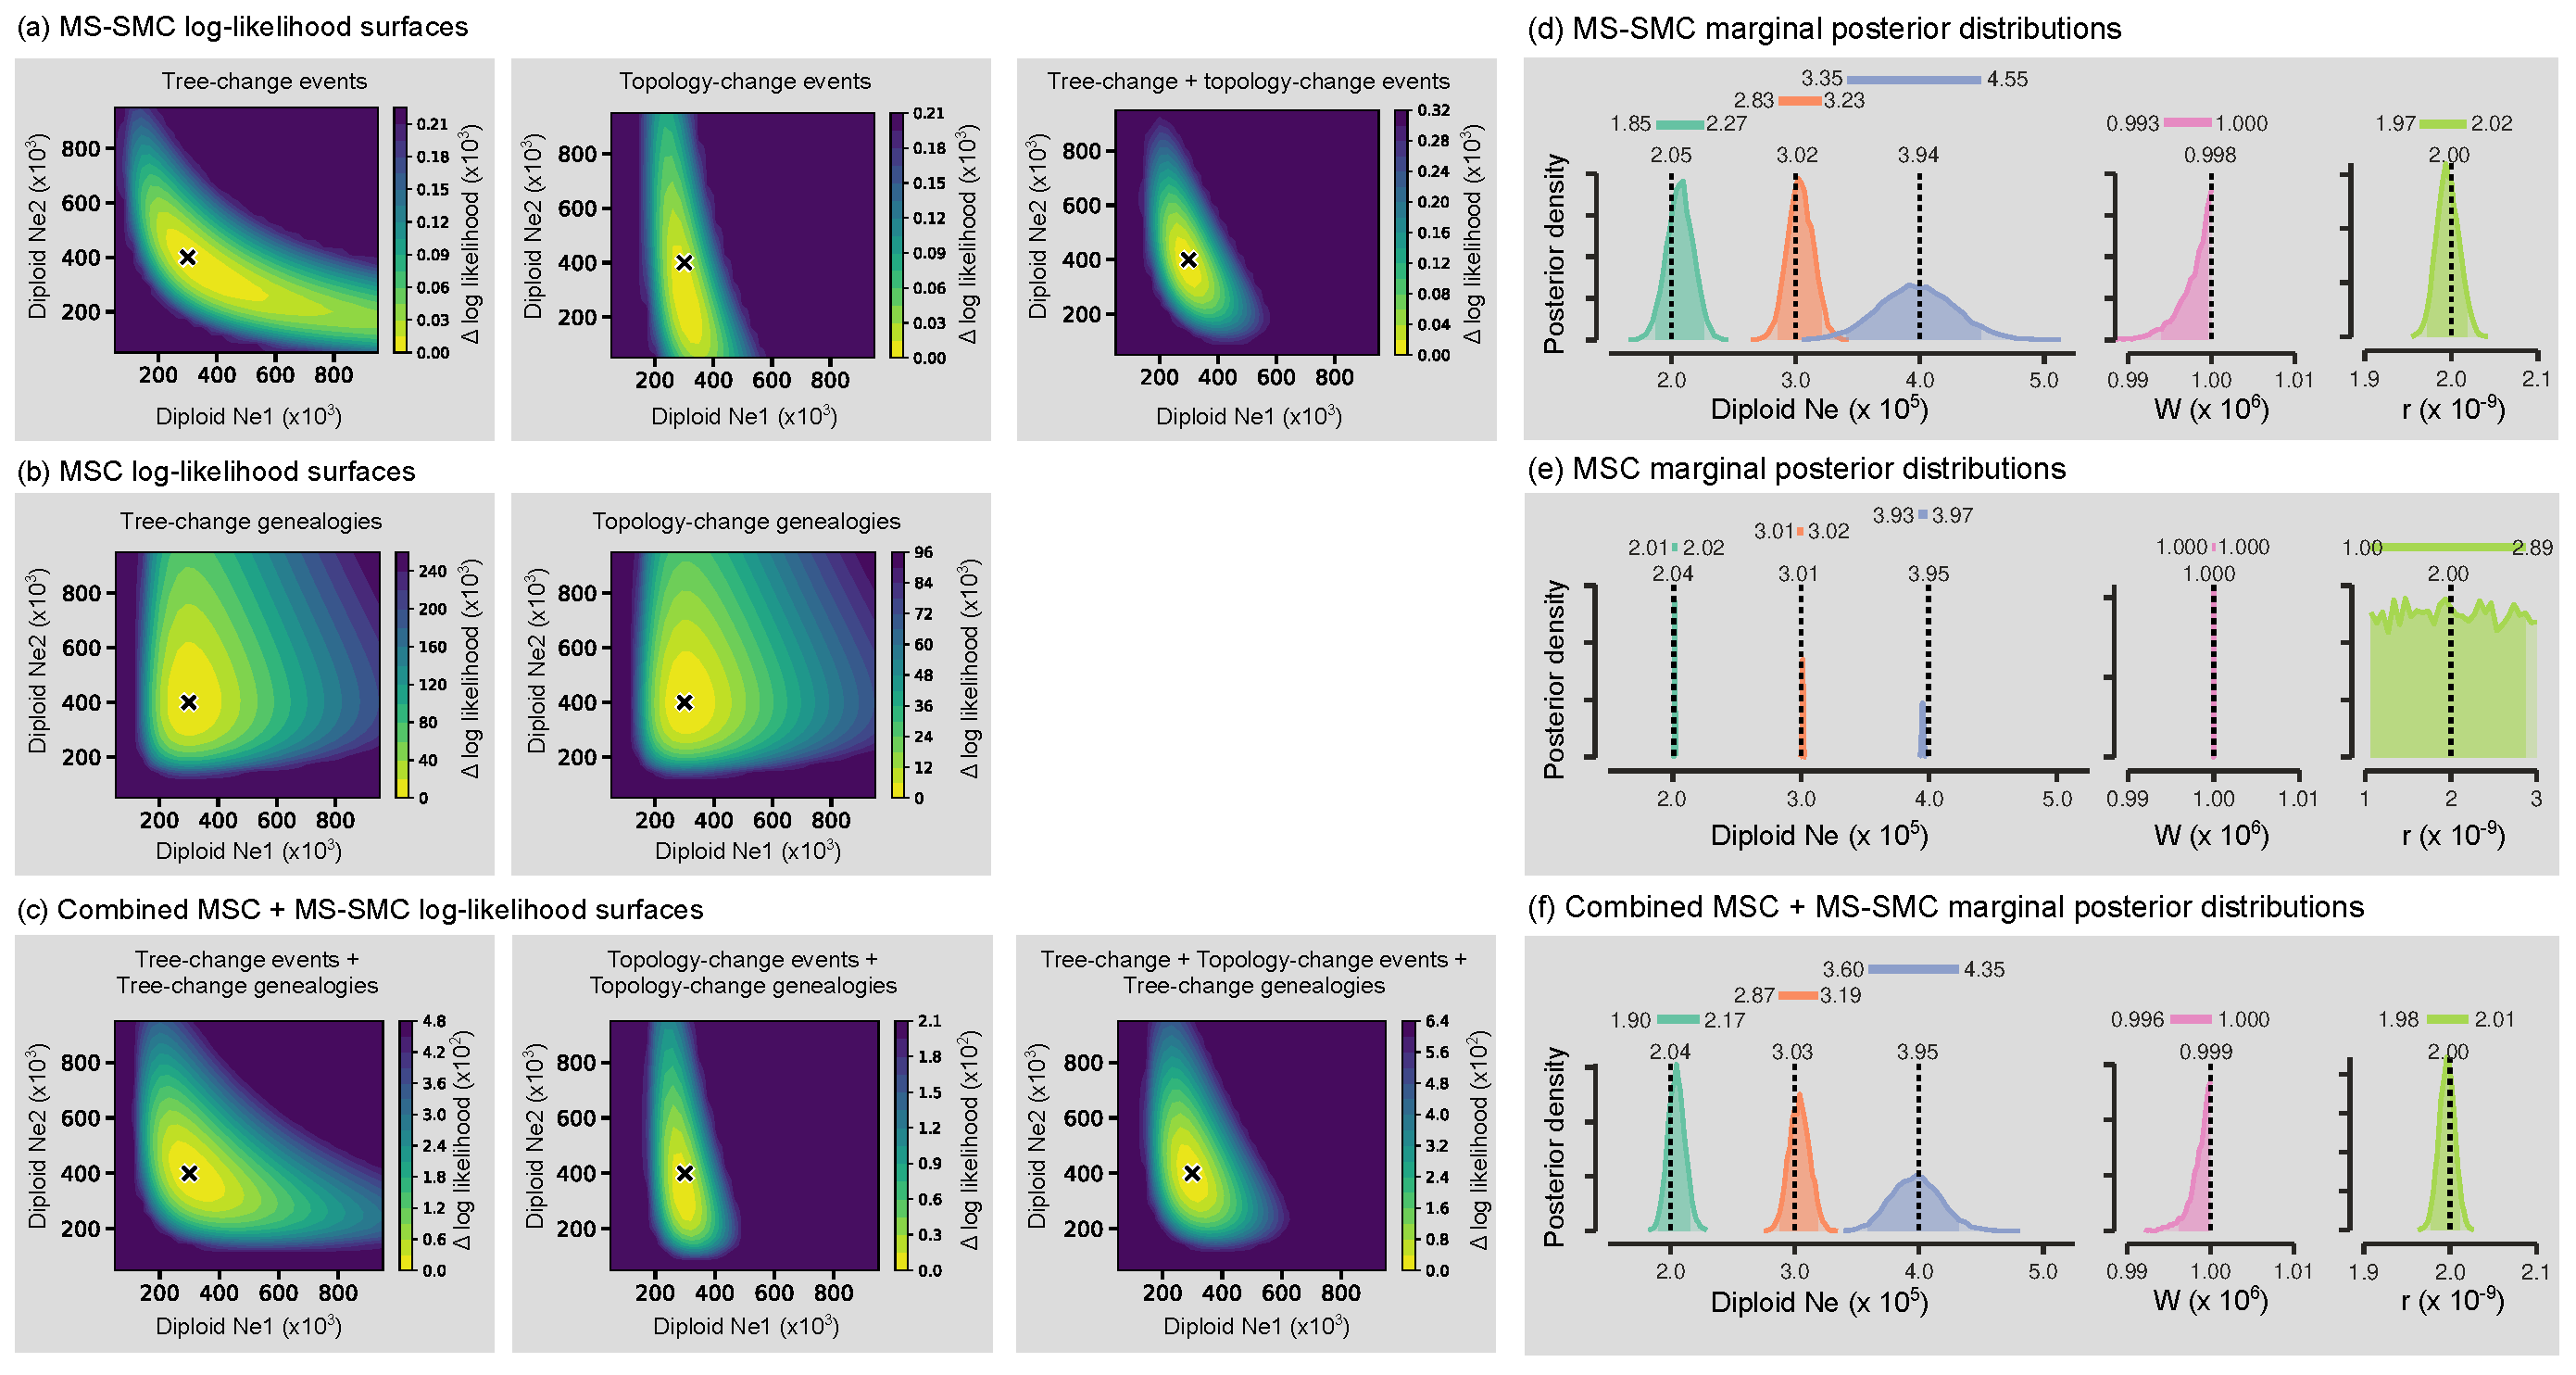
\includegraphics[width=0.99\textwidth]{figures/current/Fig8-MSC-SMC-surface-and-posterior2.pdf}
	\caption{
		A comparison of likelihood-based model inference under the MS-SMC 
		versus MSC models -- i.e., when analyzing the waiting distances of
		genealogies versus the coalescent times in genealogies, respectively.
		(a-c) Log-likelihood surfaces for parameters $N_e$1 and $N_e$2 based on 
		(a) waiting distance likelihoods computed under the MS-SMC;  
		(b) genealogy likelihoods computed under the MSC; or
		(c) the combined log-likelihoods of both types of data. 
		Note, MSC log-likelihoods are greater than MS-SMC log-likelihoods and 
		were down-weighted to a similar scale when combined.
		(d-f) The marginal posterior distributions of demographic model parameters 
		$N_e$0, $N_e$1, $N_e$2, $W$, and $r$ jointly estimated using Bayesian inference.
		True demographic model parameters are indicated by a dashed black line, above 
		which the marginal posterior mean and 95\% HPD interval are shown.
		The marginal posterior distributions correspond to model parameter inference
		from (d) combined tree-change and topology-change waiting distances;
		(e) coalescent times of genealogies between tree-change events; and 
		(f) the combined likelihoods of the data used in the previous two analyses, 
		equally weighted.
	}
	\label{fig:likelihood-posteriors}
\end{figure}


Building on the high accuracy of our MS-SMC model, as suggested by the likelihood
surfaces, we proceeded to fit a full MSC model by jointly estimating all four MSC
model parameters and the recombination rate from waiting distance data.
We applied a Bayesian approach using the Metropolis-Hastings Markov chain Monte
Carlo (MCMC) algorithm to obtain the joint posterior probability distribution of
all parameters. For this, we set uninformative uniform priors on each parameter,
using U(1e5, 1e6) for $N_e$ parameters, U(1e5, 2e6) for $W$, and U(1e-9, 3e-9) for $r$.
Four separate MCMC chains were each initiated from different random seeds, and 
each run on the same simulated ARGs from above, using the
combined likelihood of both tree-change and topology-change waiting distances.
The first 500 iterations were excluded as burn-in and used to tune the proposal 
mechanism to achieve approximately 60\% acceptance rates. From each chain, we sampled
2,000 posterior values, sampling every 10 iterations. All parameters in each chain
were assessed for convergence to confirm that ESS scores exceeded 200. The four chains 
were then joined into a single combined posterior.

Our Bayesian implementation of the MS-SMC model shows that demographic model 
parameters can be accurately estimated from waiting distance information alone.
Using waiting distances simulated under a complex two-population model with 
variable $N_e$, we recovered accurate marginal posterior estimates for all three 
$N_e$ parameters, as well as the divergence time and recombination rate 
(Fig.~\ref{fig:likelihood-posteriors}d). 
Note that the marginal posterior for the divergence time ($W$) is truncated 
slightly above the true value, since values above this do not allow for
all genealogies to be embedded in the demographic model, and were thus
rejected. 
This could be handled more appropriately by using more advanced priors on $W$. 
Across all parameters of the demographic model the true simulated values
fall within the inferred marginal 95\% highest posterior density (HPD) intervals.
This demonstrates that the tree-change and topology-change waiting distances
in an ARG contain sufficient information when evaluated under the MS-SMC model
to jointly infer all parameters of a reasonably complex demographic model.



\subsection{Combining MS-SMC and MSC likelihoods}
Finally, we compared the information contained in the lengths of 
genealogy or topology intervals (i.e., waiting distances examined under the
MS-SMC) to the information contained in the trees within those intervals 
(i.e., coalescent waiting times examined under the MSC). 
% 
Using the same simulated ARGs from above, we computed the log-likelihood
of MSC model parameters by evaluating the probabilities of only the 
genealogies between tree-change or topology-change events under the MSC,
only the waiting distances of those genealogies under the MS-SMC, 
or using both log-likelihoods combined.
% 
For MSC calculations, the probability of each genealogy was weighted 
by the length of sequence that it spanned, as this greatly improved
accuracy compared to equal weighting, and provides the same precision 
of ARG information to the MSC model as is provided to the MS-SMC model.
% 
For MSC calculations we did not combine the probabilities of genealogies
that occur between both tree-change and topology-change events, as this
would represent double-counting of the same exact trees.


The log-likelihood surface of $N_e$ parameters computed under the MSC model
was less tightly concentrated near the true values than under the MS-SMC model,
but exhibited a more round shape, suggesting less uncertainty and minimal 
correlation between parameters 
(Fig.~\ref{fig:likelihood-posteriors}a-b).
The log-likelihood of the true parameter values under the MSC model
was approximately 12 times greater than under the MS-SMC model, 
reflecting that there is generally much more information in the coalescent 
times in a genealogy than in the interval length that it spans.
Similarly, the $\Delta$log-likelihood across the examined parameter space 
was approximately three orders of magnitude greater when analyzing 
genealogies under the MSC compared to waiting distances under the MS-SMC.
% 

When evaluating model parameters based on multiple criteria, inference can 
be improved if the corresponding likelihood surfaces exhibit orthogonal or 
complementary structures, as we observed here between the MSC and MS-SMC
likelihood surfaces. 
Such differences in their shapes allow each criterion to provide unique 
information about the parameter space, which can improve the precision 
and robustness of optimization, as we showed previously for combining tree-
and topology-change waiting distances.
Here, we implemented a simple weighting scheme, 
by uniformly dividing the MSC log-likelihoods by 1000, as this 
visually led to an intermediate shape of the likelihood surface.
The resulting combined likelihood surfaces (Fig.~\ref{fig:likelihood-posteriors}c)
are more narrowly concentrated around the true values than under the MSC
model alone, and generally exhibit rounder more peaked surfaces than under
the MS-SMC model alone. 


We next applied our Bayesian joint inference framework to estimate all five 
parameters using genealogy likelihoods, or combined genealogy and waiting 
distance likelihoods. 
As before, four separate MCMC chains were run on the same ARGs from different
starting seeds, checked for convergence criteria, and then combined.
The marginal posterior distributions inferred from genealogy likelihoods 
were very narrow for all parameters except $r$, for which the MSC model
provides no information, and thus returned the prior
(Fig.~\ref{fig:likelihood-posteriors}e). 
The true values did not fall within the 95\% HPD intervals for the $N_e$
parameters, despite the posterior means being very close to the true 
values. 
This may reflect a slight bias within our MCMC implementation, or be caused
by the non-independence of genealogies being analyzed under the MSC model.
Despite this, we predicted that the combined information from genealogies
and waiting distances will provide a more accurate estimate of MSC 
parameters than from waiting distances alone, since the combined data 
tend to exhibit a more peaked and uncorrelated log-likelihood surface.
As predicted, the marginal posterior distributions inferred from these data
are more narrow and accurate than from waiting distances alone
(Fig.~\ref{fig:likelihood-posteriors}f), with all true values falling 
within the inferred 95\% HPD intervals.
This confirms that the information contained in tree- and topology-change
waiting distances is not redundant with the information contained in 
genealogy coalescent times, and that these observations can be combined
to provide additional information to evaluate the fit of an observed
or proposed ARG to a demographic model.


%%%%%%%%%%%%%%%%%%%%%%%%%%%%%%%%%%%%%%%%%%%%%%%%%%%%%%%%%%%%%%%%%%%%%%%%%%%
%%%%%%%%%%%%%%%%%%%%%%%%%%%%%%%%%%%%%%%%%%%%%%%%%%%%%%%%%%%%%%%%%%%%%%%%%%%
%%%%%%%%%%%%%%%%%%%%%%%%%%%%%%%%%%%%%%%%%%%%%%%%%%%%%%%%%%%%%%%%%%%%%%%%%%%
%%%%%%%%%%%%%%%%%%%%%%%%%%%%%%%%%%%%%%%%%%%%%%%%%%%%%%%%%%%%%%%%%%%%%%%%%%%
%%%%%%%%%%%%%%%%%%%%%%%%%%%%%%%%%%%%%%%%%%%%%%%%%%%%%%%%%%%%%%%%%%%%%%%%%%%
%%%%%%%%%%%%%%%%%%%%%%%%%%%%%%%%%%%%%%%%%%%%%%%%%%%%%%%%%%%%%%%%%%%%%%%%%%%
%%%%%%%%%%%%%%%%%%%%%%%%%%%%%%%%%%%%%%%%%%%%%%%%%%%%%%%%%%%%%%%%%%%%%%%%%%%
%%%%%%%%%%%%%%%%%%%%%%%%%%%%%%%%%%%%%%%%%%%%%%%%%%%%%%%%%%%%%%%%%%%%%%%%%%%
%%%%%%%%%%%%%%%%%%%%%%%%%%%%%%%%%%%%%%%%%%%%%%%%%%%%%%%%%%%%%%%%%%%%%%%%%%%
%%%%%%%%%%%%%%%%%%%%%%%%%%%%%%%%%%%%%%%%%%%%%%%%%%%%%%%%%%%%%%%%%%%%%%%%%%%
%%%%%%%%%%%%%%%%%%%%%%%%%%%%%%%%%%%%%%%%%%%%%%%%%%%%%%%%%%%%%%%%%%%%%%%%%%%
%%%%%%%%%%%%%%%%%%%%%%%%%%%%%%%%%%%%%%%%%%%%%%%%%%%%%%%%%%%%%%%%%%%%%%%%%%%
%%%%%%%%%%%%%%%%%%%%%%%%%%%%%%%%%%%%%%%%%%%%%%%%%%%%%%%%%%%%%%%%%%%%%%%%%%%
%%%%%%%%%%%%%%%%%%%%%%%%%%%%%%%%%%%%%%%%%%%%%%%%%%%%%%%%%%%%%%%%%%%%%%%%%%%


\section{Discussion}

Genealogical relationships vary spatially across chromosomes, reflecting 
a history of recombination between genome segments inherited from 
different ancestors. Such variation can be modeled by the sequentially 
Markov coalescent, which provides a generative process upon which 
many statistical methods have been developed \citep{mcvean2005approximating, spence_inference_2018}.
However, most applications of the SMC' remain highly limited with regard to 
the scale over which they extract information from genomes -- extending forward 
just one recombination event at a time. 
By contrast, the recent development 
by \citet{deng_distribution_2021}
of solutions for predicting 
tree- and topology-change waiting distances under the SMC' 
effectively adds two additional, longer-range sources of information for 
any position in a genome. 
In their model, these distances are a 
result of the probabilities of different phenomenological outcomes of the 
SMC' process given a genealogy embedded in a single population coalescent
model with constant $N_e$.
Here we extended this framework, deriving new solutions for the probabilities 
of tree-change and topology-change events for a genealogy embedded 
in any arbitrarily parameterized species tree model. 
While some previous studies have explored the impact of species tree parameters
on linked genealogical variation, their results have been limited to few specific
cases \citep[e.g.,][]{slatkin2006concordance}.
Our generalized solutions here lay a groundwork for 
modeling how variation in species tree parameters 
affects neutral expectations of genealogical heterogeneity across chromosomes.


The multi-species sequentially Markov coalescent (MS-SMC) is
a predictive model for the relationship between a parameterized species
tree and the length of a genomic interval over which a genealogy will 
span.
Within this framework, demographic model parameters determine
probabilities of coalescence
in species tree intervals and prevent coalescence between lineages that
are separated by species divergence events. 
This constrains the outcomes of the SMC' process, 
and thus the similarity of genealogies in sequential genomic intervals.
By categorizing the continuous outcomes of this constrained SMC' process into 
few discrete categorical outcomes, we are able to compute the probabilities of 
each type, corresponding to recombination events that delimit no change to the
genealogy, a tree-change, or a topology-change.
Using these solutions, the effect of MSC model parameters on the probability
of genealogical turnover can be computed and visualized for a single genealogy
(Fig.~\ref{fig:edge-probabilities}; Fig.~\ref{fig:figS-edge-probabilities}),
or for a distribution of genealogies simulated under an MSC model
(Fig.~\ref{fig:fig-validation}).
Using the latter approach, we demonstrated the accuracy of our solutions by
showing that the mean and variance of waiting distances predicted by our model
match closely to the results of stochastic coalescent simulations performed
on the same demographic model under the SMC' or full coalescent with 
recombination.

% Previously, lengths could only be simulated .But analytical methods are better.
A complex relationship exists between a parameterized MSC model, 
the distribution of genealogies that can arise under that model, and the 
spatial distances over which those genealogies are expected to span.
Previously, such patterns could only be examined through stochastic simulations. 
For example, \cite{mckenzie_multispecies_2020} used exhaustive simulations to
examine the effect of species tree parameters on 
the spanning length of genealogical topologies
by varying species tree length, size, and shape. 
While this approach is practical for estimating the \emph{mean} linkage across
a large set of sampled genealogies under a specific demographic model, it is
impractical for estimating the persistence of \emph{individual} genealogies. 
The analytical solutions presented here not only enable 
calculating and comparing the expected interval lengths that different 
genealogies will span given their embedding in the same species tree, 
but also enabled the development of a statistical framework for computing 
the probability of an observed waiting distance spanned by a genealogy 
as a function of the species tree model.

The multi-species coalescent is the foundation of modern phylogenetic 
methods that aim to infer a species tree as a hierarchical model within
which genealogical variation can be embedded
\citep{maddison1997gene,degnan2009gene,maddison2006inferring}.
The parameters of this model can be estimated from the distribution
of coalescent times in genealogies, and many methods have been developed
on this framework including full likelihood based analyses of molecular
sequence data \citep{rannala2003bayes}, and pseudo-likelihood or summary
based methods that analyze inferred gene tree distributions
\citep{mirarab_multispecies_2021}. 
% 
Here, we demonstrated that the parameters of a species tree model can 
alternatively be estimated from a completely new source of information,
in the form of the waiting distances between recombination events causing
a tree-change or topology-change between sequential genealogies in an ARG
(Fig.~\ref{fig:likelihood-posteriors}d).
% 
Examination of joint likelihood surfaces revealed that these two 
types of waiting distance observations provide non-redundant 
information that is complementary and orthogonal, such that when
combined they can intersect to provide more accurate estimates of 
model parameters
(Fig.~\ref{fig:likelihood-surfaces}a-b). 
% 
Similarly, although the information contained in tree- and topology-change
waiting distances is less than that contained in the coalescent times of the
same genealogies, we showed that these two sources of data can be combined,
and are also complementary and non-redundant
(Fig.~\ref{fig:likelihood-posteriors}c,f).
% 
We envision many future applications can build upon this joint framework for
evaluating the fit of ARGs to a demographic model using not only the
probabilities of genealogies within the ARG, but also the probabilities of
the spanning distances of topological features of those genealogies.
Below we describe several of these envisioned applications.

%%%%%%%%%%%%%%%%%%%%%%%%%%%%%%%%%%%%%%%%%%%%%%%%%%%%%%%%%%%%%%%%%%%%%%%%%%%%%%%%
%%%%%%%%%%%%%%%%%%%%%%%%%%%%%%%%%%%%%%%%%%%%%%%%%%%%%%%%%%%%%%%%%%%%%%%%%%%%%%%%

\subsection{The Distribution of Genealogical Variation}

One direct application of the MS-SMC model is to incorporate expectations
for the spanning lengths of genealogies into theoretical models of the
relationship between species tree models and the distribution of
genealogical variation.
% 
Consider that much of our understanding of this relationship is derived
from theoretical studies of the distribution of unlinked genealogical
topologies, without regard for differences in the expected spanning 
lengths of the topologies
\citep{degnan2005gene,degnan2006discordance}.
% 
However, as we have shown here, the same genealogy may exhibit 
very different expected spanning lengths between topology-change events
depending on the species tree model.
% 
By incorporating topology-change probabilities calculated under the
MS-SMC into theoretical models of genealogical discordance, we could shift
the focus from the frequency of occurrence of each genealogical topology, 
to the frequency of sites evolved under each topology. This would provide
a new perspective on the distribution of genealogical variation, and could
spur the development of new theoretical advances.


Another application of the MS-SMC 
is to guide the selection of appropriate locus lengths to use for gene
tree inference.
% 
For example, given a species tree hypothesis, and recombination rate, 
the probability distribution of the waiting distance between topology-change
events can be calculated for empirically inferred gene trees using our
implementation of the MS-SMC in \emph{ipcoal}. 
In theory, the locus or window size that the gene tree was inferred from
should be smaller than the mean estimated waiting distance between 
topology-change events; otherwise, the tree is likely to correspond 
to a concatenation of multiple genealogical topologies.
% 
In practice, this problem is often overlooked. The mean waiting distance
between topology-change events in multi-species datasets are often much
shorter (e.g., 10-100 bp) than the mean locus lengths of common subgenomic
markers \citep[e.g., $>$300 bp;][]{mckenzie_multispecies_2020},
and certainly much shorter than the size of genomic sliding windows 
commonly employed at genome-wide analysis scales 
\citep[e.g., 100 Kb;][]{li2019recombination}.
% 
When repeated across many loci, such concatenation artifacts bias the distribution
of gene trees, and their summary statistics, to deviate from expectations under
the MSC -- a process termed concatalescence \citep{gatesy_concatenation_2013}.
% 
The extent to which this bias affects MSC-based inference methods remains
a matter of debate.
Simulation studies under a range of species tree models and parameters
have shown that some inference methods are more sensitive to errors caused
by intra-locus recombination than others
\citep{lanier2012recombination,zhu2022simulation}, but this has not 
facilitated general recommendations that can apply to all datasets and 
methods.
% 
Topology-change probabilities calculated under the MS-SMC provide a framework
to formalize this debate around common metrics that can be computed for any 
species tree, filling a theoretical gap specifically noted by 
\citet{zhu2022simulation}.

% % The mean of
% this distribution 
% % 
% In theory, each locus or window should correspond to a
% single genealogical tree or topology.
% % 
% However, the mean waiting distance between topology-change events in
% multi-species datasets is typically much shorter (e.g., 10-100 bp) than the 
% mean locus lengths of common subgenomic markers 
% \citep[e.g., $>$300 bp;][]{mckenzie_multispecies_2020},
% and certainly much shorter than the size of genomic sliding windows 
% commonly employed at genome-wide analysis scales 
% \citep[e.g., 100 Kb;][]{li2019recombination}.
% When repeated across many loci, concatenation artifacts can cause the distribution
% of gene trees, or their summary statistics, to deviate from expectations under
% the MSC -- a process termed concatalescence \citep{gatesy_concatenation_2013}.
% % 
% The extent to which this process will bias MSC-based inferences remains
% a matter of debate.
% Simulation studies under a range of species tree models and parameters
% have shown that some inference methods are more sensitive to errors caused
% by intra-locus recombination than others
% \citep{lanier2012recombination,zhu2022simulation}, but this has not 
% facilitated general recommendations that can apply to all datasets and 
% methods.
% % 
% Topology-change probabilities calculated under the MS-SMC provide a framework
% to formalize this debate around common metrics that can be computed for any 
% species tree, filling a theoretical gap specifically noted by 
% \citet{zhu2022simulation}.


\subsection{Applications of the MS-SMC to ARG Inference}
While our demonstration of the MS-SMC framework focused on inferring
species trees from ARGs, its most impactful applications may lie 
in the inverse approach: inferring ARGs given a demographic model.
ARG inference is notoriously challenging due to the vast state
space of potential ARGs and the limited information contained
within intervals between recombination events, which complicates
the accurate reconstruction of local genealogies.
However, linkage information between neighboring intervals provides
a critical source of information that can be explicitly
modeled to propose ARGs that are statistically consistent with
an underlying evolutionary model, such as the SMC'.
% 
Nevertheless, integrating this linkage information while navigating
the immense state space of possible ARGs remains a computationally
demanding task. 
Despite these challenges, 
a number of powerful tools have been developed to efficiently 
infer ARGs and quantify uncertainty, typically through Bayesian 
posterior sampling methods
\citep{y_c_brandt_evaluation_2022,lewanski_era_2024}.


Several challenges currently limit the application and accuracy
of ARG inference at deeper phylogenetic scales. One notable limitation
is the assumption that samples originate from a single population,
which can bias estimates when the true demographic model involves 
population structure, as demonstrated in our example of model 
misspecification (Fig.~\ref{fig:likelihood-surfaces}d). 
Some methods already address this limitation, such as ARGweaver-D,
which allows users to specify a demographic model upon which ARGs 
will be conditionally sampled 
\citep{hubisz2020inference}.
% 
This approach generates ARGs with changes between sequential genealogies 
that are consistent with the SMC' process occurring within a structured
demographic model -- i.e., consistent with the MS-SMC. 
% 
However, the resulting tree- and topology-change waiting distances that 
arise in proposed ARGs are not currently incorporated into the 
likelihood calculation.
% 
We propose that our new framework, which allows computing the likelihood 
of a species tree model from the tree-change and topology-change waiting
distances in an ARG, 
could enhance both the accuracy and convergence of ARG inference by 
providing additional criteria for assessing the fit of proposed ARGs
to a species tree model.


Another potential application of the MS-SMC is to reduce the problem of 
ARG inference from inferring a genealogy and interval length between 
every recombination event, to instead infer genealogies and intervals between
only a subset of events, such as tree-change or topology-change events. 
% 
For example, topology-change events in particular leave more detectable
signatures in sequence data for identifying break points, and occur less
frequently. This could particularly benefit ARG inference above the
species-level, where the lengths of intervals between recombination events
can become very small, even to the extent that more than one 
recombination event occurs between two sequential sites, which 
would violate assumptions of the SMC' \citep{rasmussen2014genome}. 
In these scenarios, the distance between topology-change events 
will always be much longer.
% 
We do not expect that delimiting ARGs on topology-change events 
would introduce a significant bias, since as we demonstrated in 
our results, the recombination rate can still be very accurately 
inferred under the MS-SMC from the interval lengths between tree- 
and/or topology-change events alone 
(Fig.~\ref{fig:likelihood-posteriors}d). 
% 
By reducing the number of breakpoints and genealogies that must be inferred,
this would effectively reduce the complexity of the ARG inference problem, 
which could improve the efficiency and mixing of MCMC algorithms used to 
sample ARGs.


\subsection{Applications of the MS-SMC to Species Tree Inference}

In contrast to current species tree inference methods 
which tend to either ignore genetic linkage, or to discard the vast majority
of sequenced data in effort to avoid it, one could envision an alternative, 
spatially-aware phylogenetic inference framework that more effectively 
utilizes linked genomic data. This would mark a major transition in phylogenetics,
where recombination could be viewed as a source of information rather than a 
source of error. 
We see the MS-SMC as an important step in this direction. 


As a first application of the MS-SMC, we demonstrated a likelihood-based
framework to fit demographic model parameters from a known ARG based on
the distribution of tree-change and topology-change waiting distances. 
% 
When waiting distances were simulated under one demographic model, 
but used to fit parameters of a different one, 
topology-change waiting distances were particularly informative in
revealing that the incorrect model was a poor fit to the data.
% 
This suggests that the distinct tree and topology waiting 
distance distributions within ARGs generated under one species
tree model versus another can be useful for distinguishing 
between models, which is an important component of species
tree inference, network inference, and species delimitation.
% 
In this context, our likelihood-based framework for analyzing 
waiting distances could contribute to the analysis of 
linked genomic data not only for improving the inference of 
ARGs conditional on a demographic model, but also for 
comparing the fit of alternative demographic models.
% 
However, the most significant challenge to incorporating waiting distance
information into an inference framework is the fact that ARGs, and thus 
the waiting distances contained within them, are not directly observable, 
and must instead be inferred from observed sequence variation. 
% 
One solution to this problem is to evaluate demographic models by 
marginalizing over uncertainty in a posterior sample of ARGs; 
another solution is to try to bypass ARG inference altogether.
We discuss each of these approaches below.


Given the inherent complexity of ARG inference, the development 
of a joint framework for simultaneous inference of ARGs and species 
trees remains a significant challenge. 
However, if the analysis is restricted to a small number of 
competing species tree hypotheses, existing ARG inference tools
can already offer a powerful framework for demographic model 
comparison.
% 
Tools like ARGWeaver-D, for instance, not only generate posterior
samples of ARGs but also calculate the likelihood of the 
user-defined demographic model -- though note that demographic model
parameters are typically first inferred separately from unlinked
genomic data prior to this analysis and then fixed
\citep{hubisz2020inference}.
% 
While this approach does not yet scale well to large demographic
models of the size that are often investigated during species
tree inference, it can theoretically provide additional benefits
over the analysis of unlinked data, including greater power to 
infer accurate local genealogies by incorporating linkage information,
and the ability to examine local genealogies as a byproduct.
% 
In addition, by generating ARGs as a byproduct, this would 
provide the ability to analyze tree- and topology-change waiting 
distances as additional criteria for evaluating demographic 
model likelihoods. 
% 
In this context, our description above of the multiple potential
applications of the MS-SMC to improve ARG inference conditioned 
on a demographic model, also represent ways in which the MS-SMC
could improve methods for evaluating and comparing demographic models.


A situation where this may be particularly rewarding is in 
the evaluation of complex demographic models with migration, 
which are also often represented as phylogenetic networks.
% 
In network models, each genealogy can trace back a coalescent 
history through one or more paths in a model with different 
probabilities, corresponding to an embedding of the genealogy 
into one species tree model or another
\citep{wen_bayesian_2016, degnan2018modeling}. % ...
% 
When each genealogy is analyzed individually, as in the case of 
unlinked genomic data, each provides little information about the
network, and whether discordant genealogies correspond to 
introgression versus incomplete lineage sorting (ILS).
% 
Furthermore, many alternative network hypotheses are often 
unidentifiable based on the frequencies of gene tree patterns
alone \citep{solis-lemus_inferring_2016}.
% 
By contrast, ARG inference-based methods for evaluating 
structured demographic models with migration 
\citep{hubisz2020inference, guo_recombination-aware_2022}
have shown great power to infer demographic migration parameters
and distinguish between ILS and introgression in the history of
local genealogies.
% 
Given our expectation that waiting distance distributions are 
informative about alternative species tree models, we predict
that incorporating waiting distance probabilities into local ARG 
inference could further improve the power of these methods to map
genealogies into alternative coalescent paths through phylogenetic
networks.


Finally, we envision that our framework for evaluating the 
likelihood of demographic models based only on the waiting distances
in ARGs could serve as the basis for the development of demographic
inference methods for analyzing linked genome data that do 
not require ARG inference.
% 
Conceptually, a method that aims to bypass ARG inference when 
analyzing waiting distance distributions would be similar to 
the implementation of SNAPP, which aims to bypass the problem of 
gene tree inference when inferring species trees 
\citep{bryant2012inferring}.
In SNAPP, this is accomplished through a Bayesian implementation
for evaluating SNP patterns that integrates over the distribution
of genealogies that could produce each SNP.
% 
Recent work has pointed out drawbacks of this approach when applied to
pools of unlinked SNPs, since assuming independence among SNPs can 
lead to a loss of information \citep{zhu2021complexity}. 
% 
Our vision for a theoretical ARG-based extension of SNAPP would 
address this concern by specifically modeling the linkage between 
non-independent SNPs as a source of information.
% 
For example, linked SNPs that evolve on conflicting topologies can 
provide information about the probability of a topology-change event 
occurring within the distance that separates them. 
% 
Because topology-change waiting distances are inherently linked to both
the genealogy and species tree, these waiting distances could contribute
to evaluating species trees in the form of waiting distance likelihoods,
and could also possibly feedback to improve the calculation of coalescent
likelihoods, by providing information that constrains the space of 
possible genealogies at each SNP. 


\subsection{Conclusions}
We derived a generalized model for the distribution of waiting
distances between changes in a genealogical tree or topology, 
given a parameterized species tree model.
% 
Beyond its applications for species tree and ARG inference, 
this framework provides a foundation for establishing neutral 
expectation for the spatial turnover of genealogical 
relationships across a genome.
% 
Such expectations are particularly useful for identifying
deviations caused by model violations, such as introgression,
or non-neutral processes like selection.
% 
With genome-scale data now widely available, gene tree inference
is commonly performed in sliding windows across a genome to examine
the spatial distributions of topological relationships, where
deviations of patterns from a genome-wide average are interpreted
as evidence of selection or introgression
\citep{martin_exploring_2017,zhang2016genome,li2019recombination}.
% 
These interpretations are typically based on the lengths of genomic
intervals over which particular topologies are observed, 
sometimes in relation to an estimated recombination map.
% 
We suggest that such conclusions should be critically evaluated
when made without reference to a null model-based expectation. 
% 
Our results show that neutral expectations for waiting distances between 
genealogy changes can exhibit considerable variance, and that this 
variance is spatially auto-correlated, meaning that a clade or topology
may persist over long intervals of a genome simply by chance.
% 
By providing analytical solutions for the distribution of the waiting
distance to tree and topology changes under a demographic model, 
our results provide a new statistical framework for evaluating 
local genealogical patterns.



\subsection{Acknowledgements}
This work was supported by the National Science Foundation 
(NSF DEB-2046813 awarded to D.A.R.E. and NSF Graduate Research Fellowship 
DGE 16-44869 awarded to P.F.M.). Thanks to Yun Deng for discussion
on waiting distance methods, to Jerome Kelleher for and two anonymous 
reviewers for suggestions that improved the manuscript, and to members of 
the Eaton Lab for valuable feedback.

\subsection{Data Availability}
Code to calculate MS-SMC probabilities and waiting distances is 
implemented in the Python package \emph{ipcoal} 
(\url{https://github.com/eaton-lab/ipcoal}). 
Jupyter notebooks demonstrating the MS-SMC calculations and with 
reproducible code used for validations in this study are available
at \url{https://github.com/eaton-lab/waiting-distance-code}. Notebooks
and code were also archived in DRYAD at
\url{https://doi.org/10.5061/dryad.jdfn2z3n7}.
(Reviewer Sharelink: 
\url{http://datadryad.org/stash/share/_4s04af8qeWaVNIzQGs0klGrMEFBhoqlWIxgu66h6WA}).


\bibliographystyle{ecol_let}
\bibliography{references}  

%%% Uncomment this line and comment out the ``thebibliography'' section below to use the external .bib file (using bibtex) .


%%% Uncomment this section and comment out the \bibliography{references} line above to use inline references.
% \begin{thebibliography}{1}

% 	\bibitem{kour2014real}
% 	George Kour and Raid Saabne.
% 	\newblock Real-time segmentation of on-line handwritten arabic script.
% 	\newblock In {\em Frontiers in Handwriting Recognition (ICFHR), 2014 14th
% 			International Conference on}, pages 417--422. IEEE, 2014.

% 	\bibitem{kour2014fast}
% 	George Kour and Raid Saabne.
% 	\newblock Fast classification of handwritten on-line arabic characters.
% 	\newblock In {\em Soft Computing and Pattern Recognition (SoCPaR), 2014 6th
% 			International Conference of}, pages 312--318. IEEE, 2014.

% 	\bibitem{hadash2018estimate}
% 	Guy Hadash, Einat Kermany, Boaz Carmeli, Ofer Lavi, George Kour, and Alon
% 	Jacovi.
% 	\newblock Estimate and replace: A novel approach to integrating deep neural
% 	networks with existing applications.
% 	\newblock {\em arXiv preprint arXiv:1804.09028}, 2018.

%\end{thebibliography}



%%%%%%%%%%%%%%%%%%%%%%%%%%%%%%%%%%%%%%%%%%%%%%%%%%%%%%%%%%%%%%%%%%%%%%%%%%%
%%%%%%%%%%%%%%%%%%%%%%%%%%%%%%%%%%%%%%%%%%%%%%%%%%%%%%%%%%%%%%%%%%%%%%%%%%%
%%%%%%%%%%%%%%%%%%%%%%%%%%%%%%%%%%%%%%%%%%%%%%%%%%%%%%%%%%%%%%%%%%%%%%%%%%%
%%%%%%%%%%%%%%%%%%%%%%%%%%%%%%%%%%%%%%%%%%%%%%%%%%%%%%%%%%%%%%%%%%%%%%%%%%%
%%%%%%%%%%%%%%%%%%%%%%%%%%%%%%%%%%%%%%%%%%%%%%%%%%%%%%%%%%%%%%%%%%%%%%%%%%%
%%%%%%%%%%%%%%%%%%%%%%%%%%%%%%%%%%%%%%%%%%%%%%%%%%%%%%%%%%%%%%%%%%%%%%%%%%%
%%%%%%%%%%%%%%%%%%%%%%%%%%%%%%%%%%%%%%%%%%%%%%%%%%%%%%%%%%%%%%%%%%%%%%%%%%%



\newpage

\beginsupplement
\section{Supplementary Information}

\setcounter{equation}{0}
\renewcommand{\theequation}{S\arabic{equation}}

\subsection{Supplementary Figures}

\begin{figure}[p]
	\centering
	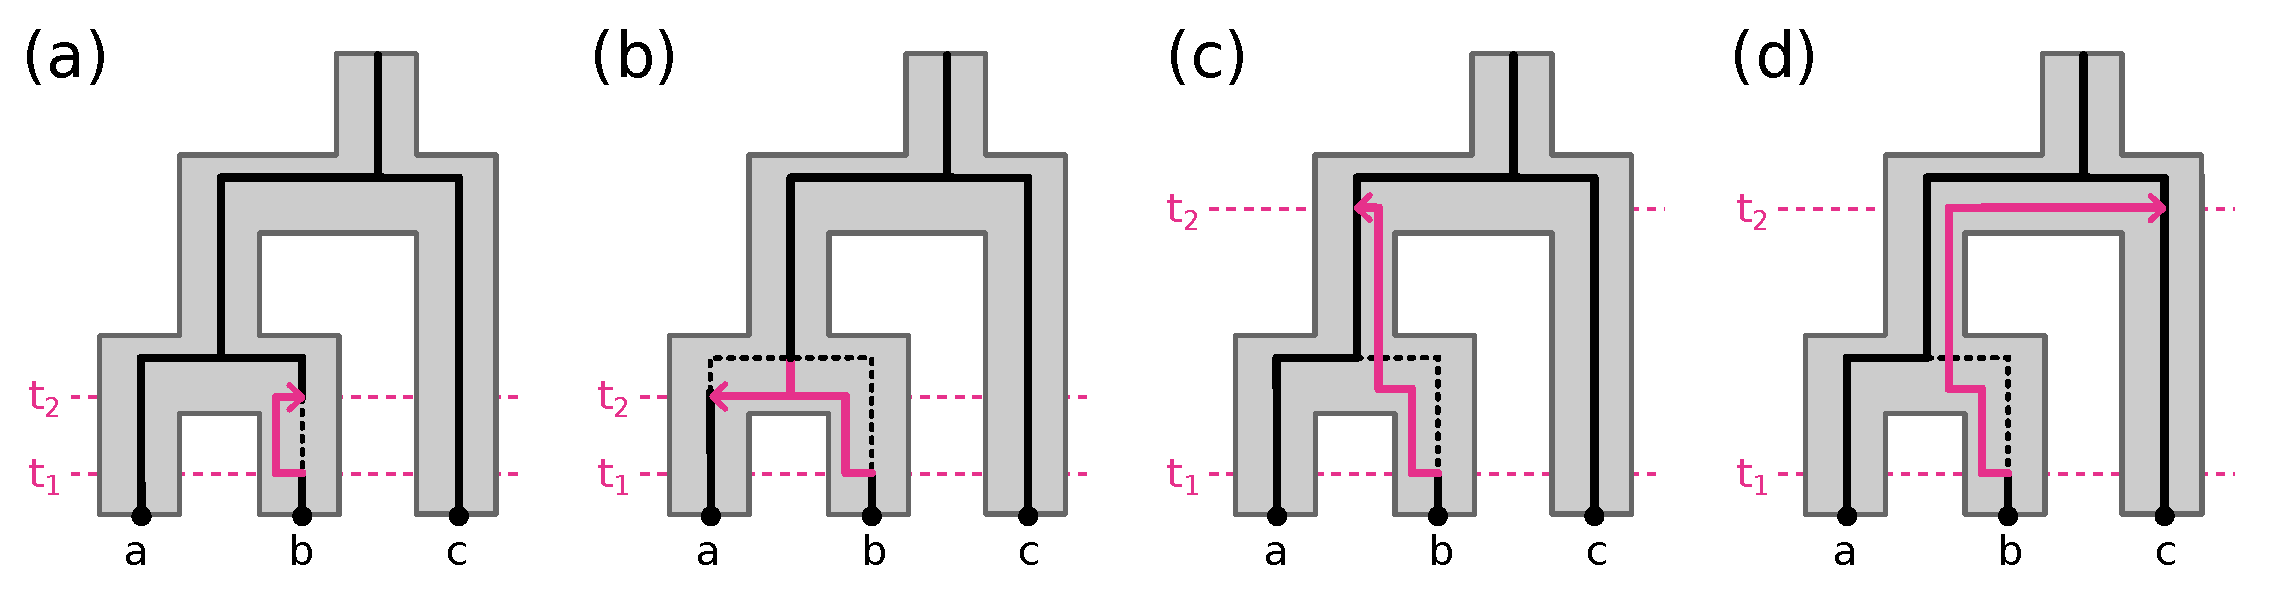
\includegraphics[width=0.9\textwidth]{figures/current/FigS1-recomb-types.pdf}
	\caption{
		Four categories of outcomes from a recombination event occurring on a
		%genealogy at time t$_1$ and the detached subtree re-coalescing with
		genealogy at time t$_1$, dictated by random subtree re-coalescence with
		a remaining lineage under the SMC' process at time t$_2$. (a) The
		detached subtree re-coalesces with the original lineage from which it
		was detached, leading to no change between the starting genealogy and 
		subsequent genealogy. (b) The detached subtree re-coalesces with its
		sibling lineage prior to their previous coalescence, leading to a shortening
		of their coalescence time. (c) The detached subtree re-coalesces with
		its parent lineage, leading to a lengthening of the coalescent time 
		between the detached subtree lineage and its sibling lineage. (d) The
		detached subtree re-coalesces with a lineage other than itself, its sibling,
		or its parent lineage, leading to a topology-change. 
	}
     \label{fig:figS-recomb-types}
\end{figure}


\begin{figure}[p]
	\centering
	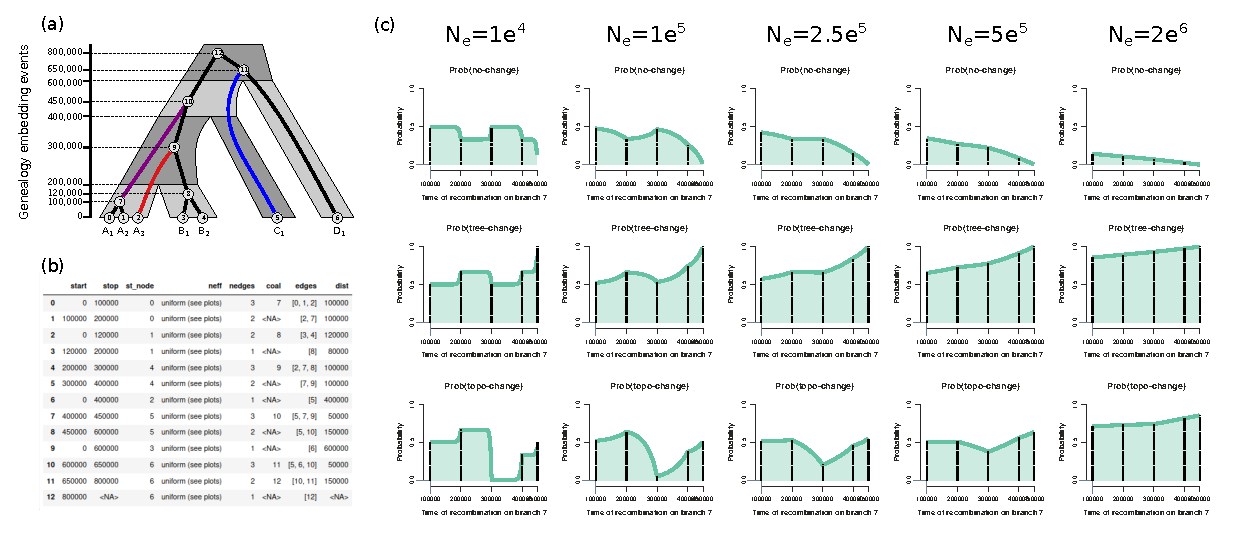
\includegraphics[width=0.99\textwidth]{figures/Fig-S2-edge-probabilities.pdf}	
	\caption{
		Probabilities of different recombination event outcomes for a selected 
		genealogy edge as a function of the time at which recombination occurs 
		and of the constant effective population size.
		(a) An MSC model with edge lengths in units of generations and an example
		genealogy embedded. (b) An genealogy embedding table for the example MSC
		model and genealogy. (c) Probabilities of different recombination event
		outcomes across genealogy edge 7. When $N_e$ is low, probabilities are 
		nearly constant with respect to time within each interval since re-coalescence in later intervals
		is unlikely. When $N_e$ is high, probabilities change nearly monotonically 
		across the length of an edge since population structure does little
		to constrain the time of re-coalescence.
	}
     \label{fig:figS-edge-probabilities}
\end{figure}


\begin{figure}[p]
	\centering
	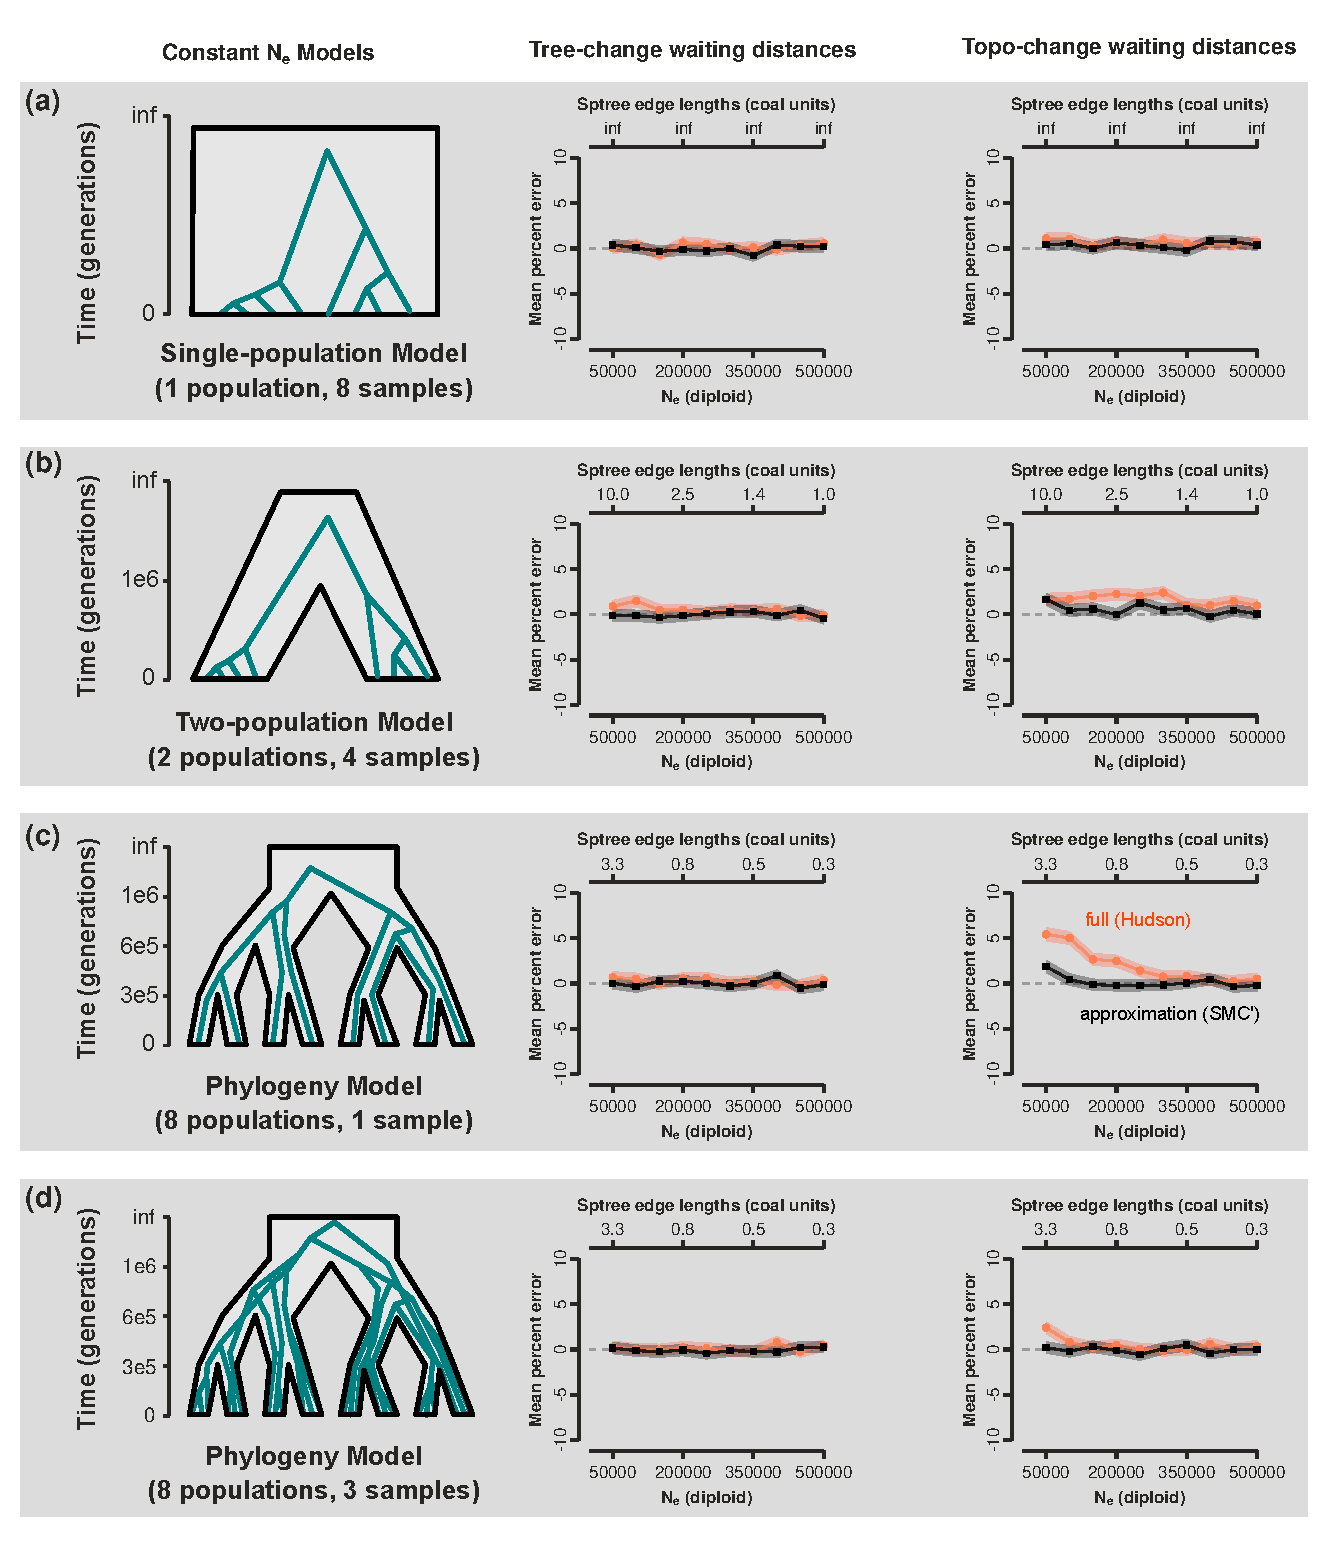
\includegraphics[width=0.79\textwidth]{figures/current/FigSY-smc-approx-bias.pdf}	
	\caption{
		Error in the expected waiting distances to tree or topology-change events 
		calculated under the MS-SMC.
		Error was measured as (observed - expected) / expected, where observed is the 
		spanning distance of the first genealogy in a tree sequence until the next 
		tree or topology-change event, and expected is the predicted waiting distance
		for the first genealogy until each event type given its embedding in the 
		species tree model.
		Tree sequences were simulated for different demographic models across a range 
		of parameter settings for $N_e$, and under two different ancestry models
		(SMC'=black; full coalescent with recombination (Hudson)=orange).
		(a-d) Estimated tree-change waiting distances exhibit very little error across
		all models and parameters tested. Estimated topology-change waiting distances
		exhibit elevated error at low $N_e$ values in highly structured models, when
		the probability of a topology-change event is very low.
		(c) The error between analytical predictions and simulated data was greatest 
		when the data were simulated under the full coalescent with recombination. 
		(d) When more genomes are sampled per lineage the magnitude of error is greatly
		reduced.
	}
	\label{fig:figS-bias-smc}
\end{figure}



\begin{figure}[p]
	\centering
	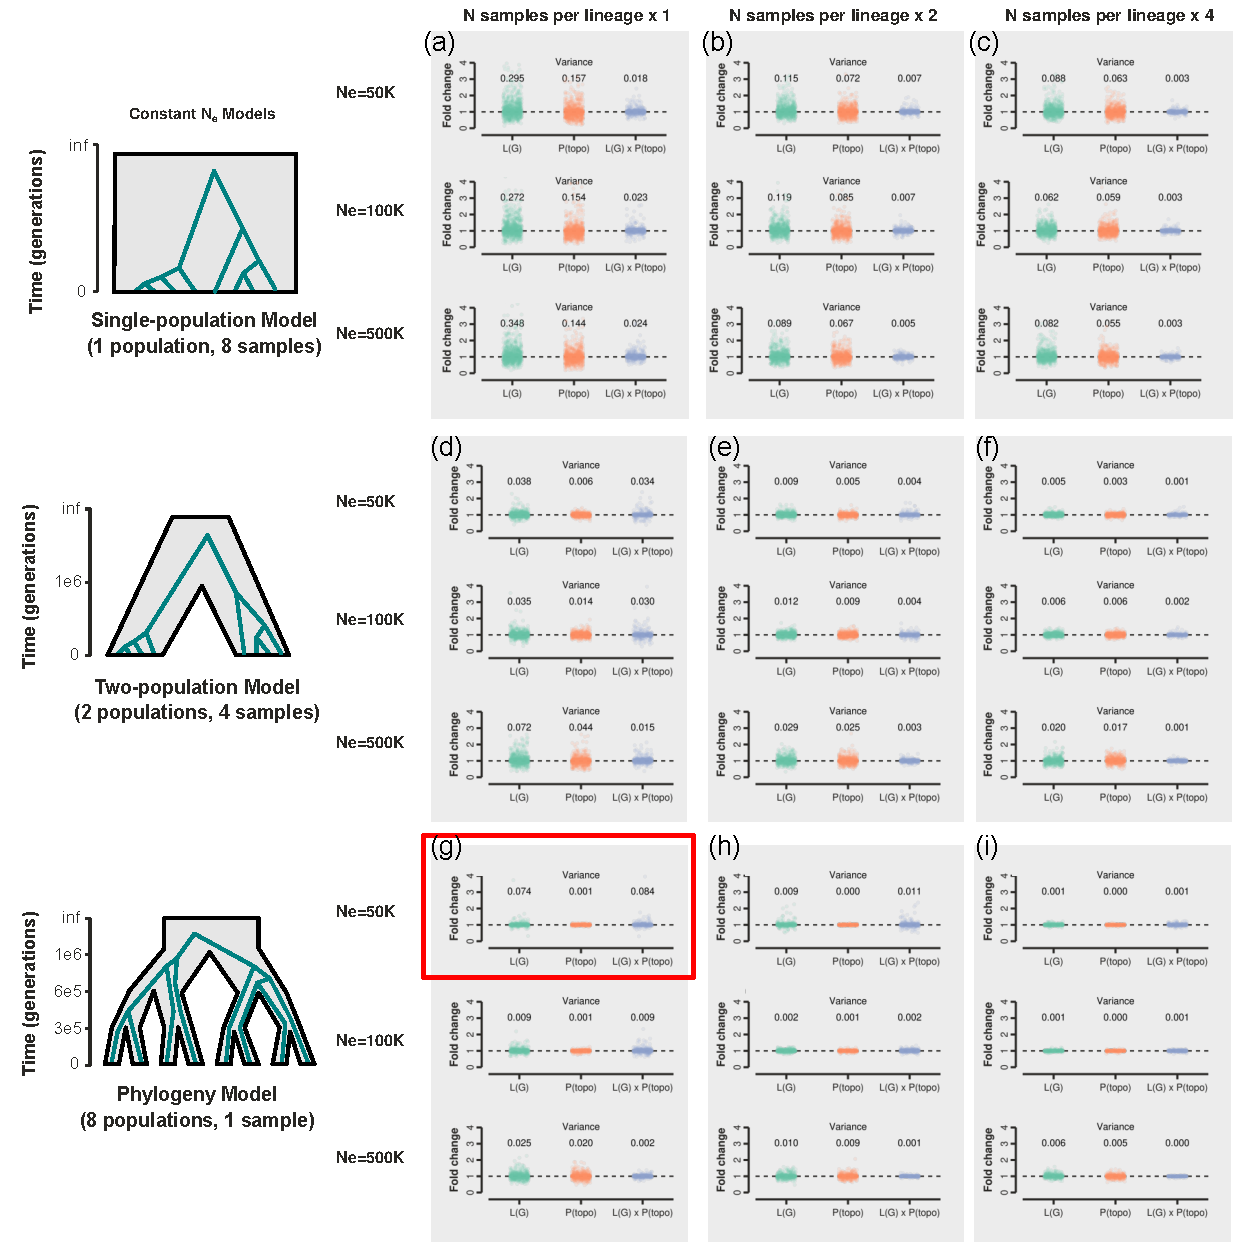
\includegraphics[width=0.99\textwidth]{figures/current/FigS-bias-fold-topo-first-2.pdf}
	\caption{
		Variation between the first and second genealogies within topology-change 
		intervals, and its impact on estimated waiting distances.
		Results are shown for 1K tree sequences simulated across a range of 
		demographic models, $N_e$ values, and numbers of genomes sampled per lineage.
		% 
		For each scenario, plots show the distribution of fold-change differences
		between the first and second genealogies in summed edge lengths (L(G)),
		the probability of a topology change (P(topo)), and the product of these
		metrics. The variance is shown above each distribution.
		% 
		(a-c) Single population demographic models consistently show high variance
		in the fold-change of each individual metric, but low variance in the
		fold-change of the product.
		(d-i) The two-population and phylogeny models typically exhibit less 
		variance, except in the lowest $N_e$ scenarios (e.g., red rectangle),
		where the product sometimes exhibits higher variance in fold-change.
		% 
		This suggests that the potential for tree-change events occurring within a 
		topology-change interval to bias estimates of the waiting distance to a
		topology-change, is only a concern in scenarios where topology-change events
		are very unlikely. (e,f,h,i) Sampling more genomes per lineage greatly 
		reduces this bias.
	}
     \label{fig:figS-bias-topo-first}
\end{figure}


\begin{figure}[p]
	\centering
	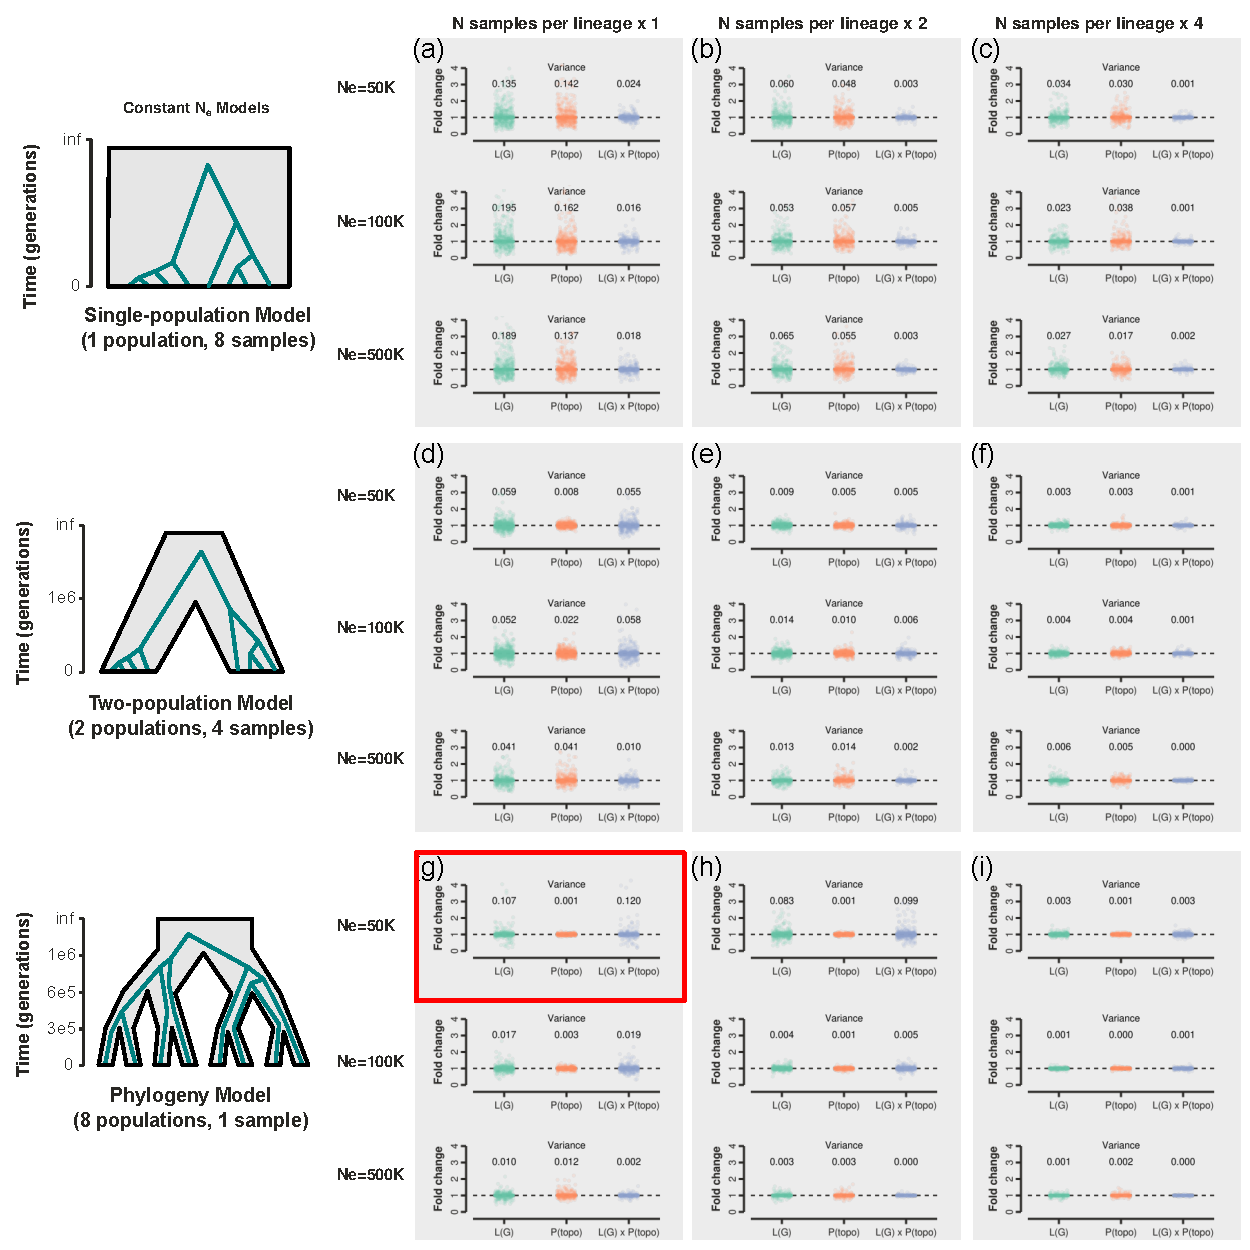
\includegraphics[width=0.99\textwidth]{figures/current/FigS-bias-fold-topo-last-2.pdf}
	\caption{
		Variation between the first and last genealogies within topology-change 
		intervals, and its impact on estimated waiting distances.
		Results are shown for 1K tree sequences simulated across a range of 
		demographic models, $N_e$ values, and numbers of genomes sampled per lineage.
		% 
		For each scenario, plots show the distribution of fold-change differences
		between the first and last genealogies in summed edge lengths (L(G)),
		the probability of a topology change (P(topo)), and the product of these
		metrics. The variance is shown above each distribution.
		% 
		(a-c) Single population demographic models consistently show high variance
		in the fold-change of each individual metric, but low variance in the
		fold-change of the product.
		(d-i) The two-population and phylogeny models typically exhibit less 
		variance, except in the lowest $N_e$ scenarios (e.g., red rectangle),
		where the product sometimes exhibits higher variance in fold-change.
		% 
		This suggests that the potential for tree-change events occurring within a 
		topology-change interval to bias estimates of the waiting distance to a
		topology-change, is only a concern in scenarios where topology-change events
		are very unlikely. (e,f,h,i) Sampling more genomes per lineage greatly 
		reduces this bias.		
	}
     \label{fig:figS-bias-topo-last}
\end{figure}




\begin{figure}[p]
	\centering
	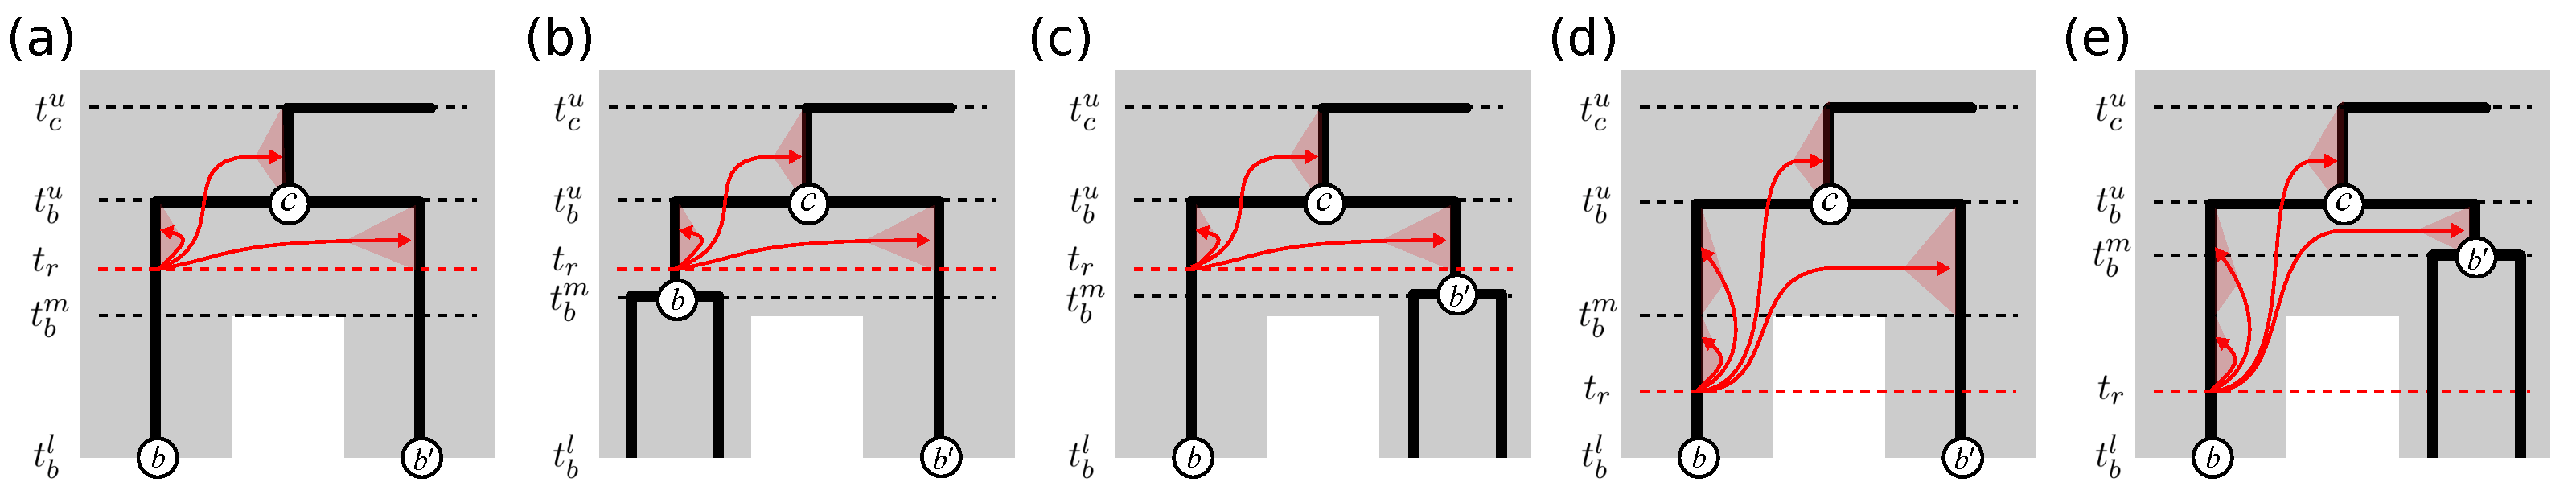
\includegraphics[width=0.95\textwidth]{figures/FigS-tbm.pdf}
	\caption{
		Calculating the probability that recombination on genealogy branch 
		$b$ leads to a topology change involves summing over the probabilities 
		that the detached lineage does not re-coalesce with either
		itself, its sibling, or its parent ($b$, $b'$ or $c$, respectively). 
		The possibility of a tree-change outcome (e.g., shortened coalescent 
		time) is restricted until the lowest shared interval between $b$ and 
		$b'$, designated at time $t_m$. Opportunities for such events could be
		constrained by species divergences -- as in (a) and (d) -- or by the timing of 
		prior coalescence events generating each branch -- as in (b), (c), and (e). 
		The possibility that recombination ($t_r$) occurs prior
		to $t_m$ leads to the two ordered sets of intervals used in 
		equations 11 and 12.
	}
	\label{fig:figS-tbm}
\end{figure}


\begin{figure}[p]
	\centering
	\includegraphics[width=0.95\textwidth]{figures/current/FigS6-equations}
	\caption{A step-by-step calculation of the probability of a tree-unchanged 
	event under the MS-SMC given a species tree and genealogy.
	}
	\label{fig:figS-tree-equations}
\end{figure}


\begin{figure}[p]
	\centering
	\includegraphics[width=0.95\textwidth]{figures/current/FigS7-equations-topo}
	\caption{A step-by-step calculation of the probability of a topology-unchanged 
	event under the MS-SMC given a species tree and genealogy.
	}
	\label{fig:figS-topo-equations}
\end{figure}


\begin{table}[p]
\centering
\caption{\label{tab:table-notation} 
	Summary of variables used in waiting distance equations. 
}
\begin{tabular}[t]{ |c|l| }
	\toprule
	Variable & Description \\
	\midrule
	$\mathcal{S}$    & An MSC model with topology, divergence times and effective population sizes. \\
	$\mathcal{G}$    & A genealogy that can be embedded in $\mathcal{S}$. \\
	$L(\mathcal{G})$ & Sum of edge lengths of genealogy $\mathcal{G}$. \\
	$b$ 			  & A focal branch in $\mathcal{G}$. \\
	$i$              & Interval in the genealogy embedding table in which recombination occurs.\\
	$\mathcal{I}_b$  & Ordered set of intervals on branch $b$.\\
	$\mathcal{I}_{c}$   & Ordered set of intervals on branch $c$, the parent of branch $b$.\\
	$\mathcal{I}_{bc}$  & Ordered union of sets $\mathcal{I}_{b}$ and $\mathcal{I}_{c}$.\\
	$\mathcal{J}_b(i)$  & Ordered set of intervals above $i$ on branch $b$.\\	
	$\mathcal{Q}_b(i,j)$ & Ordered set of intervals above $i$ and below $j$ on branch $b$.\\
	$\mathcal{K}(b,t)$ & Number of edges of $\mathcal{G}$ in the interval containing branch $b$ at time $t$.\\
	$k_x$              & Number of edges of $\mathcal{G}$ in interval $x$; piece-wise constant of $A(b,t)$.\\
	$\mathcal{N}(b,t)$ & Diploid effective population size in the interval containing branch $b$ at time $t$.\\
	$n_x$              & Diploid effective population size in interval $x$; piece-wise constant of $N(b,t)$. \\
	$t_r$		& Time of a recombination event, in generations. \\
	$\sigma_x$     & The lower boundary of interval $x$, in generations. \\
	$\mu_x$        & The upper boundary of interval $x$, in generations. \\	
	$d_x$          & The length of interval $x$, in generations. \\
	$t_b^l$        & The lower boundary of branch $b$, in generations. \\
	$t_b^u$        & The upper boundary of branch $b$, in generations. \\
	$t_b^m$        & The time at which a focal branch $b$ is able to coalesce with its sibling branch. \\
	% $m$            & Index of an interval in the genealogy embedding table with lower boundary $t_b^m$. \\
	$\mathcal{M}_b$  & Ordered set of intervals above $t_b^m$ on branch $b$.\\
	$\mathcal{L}_b$  & Ordered set of intervals below $t_b^m$ on branch $b$.\\	
	% $\mathcal{I}_b$  & The number of intervals containing branch $b$. \\
	\bottomrule
\end{tabular}
\end{table}



\newpage


\subsection{Investigating bias in MS-SMC predictions}
The MS-SMC harbors two potential sources of bias, the first stemming from 
assumptions of the SMC' approximation and the second from the 
potential inhomogeneity among genealogies that can exist 
between topology-change events.
% 
We examined both of these sources of error through comparison to stochastic
simulations and found that their effects are generally negligible,
and that structured demographic models do not exhibit 
greater error than a single-population model under most scenarios.


\subsubsection{Bias associated with the SMC' approximation}
To investigate 
the extent to which the SMC' approximation leads to errors in waiting
distance estimation, 
we repeated the simulations from our validation scenario using the SMC'
model (msprime setting "ancestry\_model=smc\_prime") as opposed to the 
full coalescent with recombination model ("ancestry\_model=hudson") that
we used previously.
% 
We expect that waiting distances in simulations under the SMC' will match 
our analytical predictions more closely than the waiting distances in 
simulations under the full coalescent with recombination, since our MS-SMC
model relies on the assumptions of the SMC'.
% % 
For each simulated tree sequence we calculated the expected waiting distance to 
a tree or topology-change event given the starting genealogy and species tree, 
and compared this to the observed waiting distance to each event type for the
starting genealogy in the simulation.
% 
We measured the percent error for each genealogy
as 100 $\times$ (simulated waiting distance - expected waiting distance) / expected waiting distance.
This was repeated across 100K tree sequences for each simulation setting, 
and the mean and standard error were calculated.

The error in our analytical predictions was very low across all demographic
models and parameter settings tested, regardless of whether data were simulated
under the SMC' approximation or not
(Fig.~\ref{fig:figS-bias-smc}). 
% 
The mean percent error in estimated tree-change waiting distances 
rarely exceeded 1\%, while the error in estimated topology-change 
waiting distances varied depending on the demographic and simulation 
models.
% 
The error in estimated topology-change waiting distances was always
$<$5\% for data simulated under the SMC', and only exceeded 5\% in
one scenario tested for simulations under the full coalescent with
recombination. This scenario represents an extreme case, in the form of
a "Phylogeny Model" with only a single sample per species, and very low 
Ne, such that genealogical discordance is very low. This leads to very 
long expected waiting distances between topology events, and very high 
variance in the simulated outcomes (Fig.~\ref{fig:figS-bias-smc}c). 
By simply increasing the number of samples per lineage, such that 
topology-change events can occur not only between lineages, but also 
within them, this error is reduced to approximately 2\% for the full 
coalescent with recombination, and nearly zero for SMC' data 
(Fig.~\ref{fig:figS-bias-smc}d). 


Although tree-change waiting distances did not exhibit consistent errors,
the error in estimated topology-change waiting distances, when present,
was consistently in the direction of being under-estimated. The fact that
this bias is not observed in the distance to tree-change events, but only
for topology-change events, suggests that the SMC' approximation has
little effect on the accuracy of estimation for an individual genealogy,
but can lead to more detectable errors when compounded over many tree-change
events occurring between a topology-change event.
% 
In other words, the SMC' approximation does not introduce a significant
bias on its own, but does contribute to increased error in topology-change 
change waiting distances through its interaction with a second source of error,
the inhomogeneity of genealogies between topology-change events (examined
further below). 
% 
We expect that the reason this bias tends to occur in the direction
of under-estimated waiting distances to a topology-change is because 
the intervening tree-change events can cause the genealogy to enter a 
space where the probability of a topology-change is much less likely 
than it was on the tree at the start of the interval. 


\subsubsection{Bias associated with inhomogeneity between topology-change events}

To investigate the impact of genealogical variation within a topology-change interval
on the accuracy of its estimated waiting distance, we measured how much genealogies vary
within these intervals, and how much this impacts probabilities of topology-change.
% 
Because topology-change waiting distances are calculated based on the genealogy
at the start of an interval, we compared the first genealogy to both the second
and last genealogy in each interval.
% 
For each tree we calculated the genealogy length ($L(\mathcal{G})$), 
the probability of a topology-change given $\mathcal{G}$ and $\mathcal{S}$,
and the product of these two metrics, which equates to the waiting distance 
rate parameter (equations 7, 8, 10).
% 
\citet{deng_distribution_2021} noted that for a single population with constant $N_e$
there is an inverse relationship between genealogy length and the probability of a 
topology change, such that their product exhibits little variation even if genealogies
vary across an interval.
% 
It was not clear whether this is also true for an MSC model, since the embedding of
a genealogy into the species tree affects the probability of a topology change in 
addition to the edge lengths of the genealogy. 
% 


Therefore, we examined genealogical variation across three demographic models, 
at three different values for $N_e$, and for different numbers of genomes sampled
per population. We simulated 1,000 tree sequences for each scenario using the 
coalescent with recombination ancestry model. 
% 
For each tree sequence we extracted information from one topology-change interval. 
To select the interval we advanced to the first interval after the first topology-change 
event that included at least one tree-change event within it.
For this interval we measured $L(\mathcal{G})$, 
$\mathbb{P}(\textrm{topology-change}| \mathcal{S}, \mathcal{G})$ and their
product, for the first genealogy, second genealogy, and last genealogy in the interval.
We measured the fold-change for each variable between the first and second 
genealogies, and between the first and last genealogies.
% 


Across all simulations our results confirm and extend the conclusions of 
\citet{deng_distribution_2021}, showing that although $L(\mathcal{G})$ 
and $\mathbb{P}$ can both exhibit high variance in fold-change between the 
first and second genealogies in an interval (Fig.~\ref{fig:figS-bias-topo-first}), 
and between the first and last genealogies in an interval (Fig.~\ref{fig:figS-bias-topo-last}),
the product of these two metrics almost always exhibits lower variance in
fold-change, and is centered on one.
% 
In a single population model the variance in the fold-change of the product of
these two metrics was approximately 0.02, and did not vary with $N_e$, or 
depending on whether we compared the first and second, or first and last
trees in an interval. The variance in the product was reduced by nearly 
an order of magnitude when the number of genomes sampled was increased 
(Fig.~\ref{fig:figS-bias-topo-first}a-c,\ref{fig:figS-bias-topo-last}a-c).
We can conclude that genealogical heterogeneity has a very small effect
on estimated waiting distances to topology-changes in a single population model.

% 
In the two-population and phylogeny models the variance in the fold change of 
$L(\mathcal{G})$, $\mathbb{P}$, and their product was strongly affected by the
model $N_e$, and consistently smaller between the first and second genealogy, 
than between the first and last genealogy in an interval.
(Fig.~\ref{fig:figS-bias-topo-first}d-i,\ref{fig:figS-bias-topo-last}d-i). 
% 
Despite this, the variance in fold-change of the product was of a similar
magnitude or lower than in the single-population model across nearly 
all of the multi-species scenarios tested.
% 
The only exception is the extreme case noted previously, representing the
Phylogeny Model with only a single genome sampled per tip, examined at the 
lowest $N_e$ value (50K), where the probability of a topology-change is 
very low because the probability of coalescence within each species tree
interval is very high
(Fig.~\ref{fig:figS-bias-topo-first}g,\ref{fig:figS-bias-topo-last}g).
% 
At only slightly higher values of $N_e$ (100K) the variance in the fold-change
difference between trees is of a similar magnitude, or lower, than that
seen in the single population model. 
% 
Thus, we can conclude that genealogical heterogeneity has only a small 
effect on estimated waiting distances to topology-changes in most 
multi-species coalescent models, but that care should be taken when 
interpreting MS-SMC estimated waiting distances to topology-changes estimated
on datasets that lack genealogical discordance. 
% 
As noted previously, simply increasing the number of sampled genomes
per lineage, to a number that allows topology-change events to occur both
within and between lineages, reduces the variation in topology-change 
probabilities across within intervals to negligible values
(Fig.~\ref{fig:figS-bias-topo-first}i,\ref{fig:figS-bias-topo-last}i).



\section{Appendix: Derivations}

\subsection{Notation}

Information from the genealogy embedding table (described in the following paragraph) can be used 
in equations that 
calculate the 
probabilities of no-change, tree-change, and topology-change events under the 
MS-SMC. These equations, described throughout rest of the Appendix, use the terms defined in 
Table~\ref{tab:table-notation}. 
A parameterized species tree, $\mathcal{S}$, is a multispecies coalescent 
model in which a set of isolated populations are related by a bifurcating
tree topology. Divergence times between lineages are in units of generations, 
and each edge (species tree interval) can be associated with a different constant 
diploid effective population size ($N_e$). 
A genealogy, $\mathcal{G}$, represents the genealogical relationships -- composing
a topology and coalescent times in units of generations -- for a set 
of sampled gene copies at some position in their genomes. A genealogy can be 
embedded in a species tree if the coalescent times between sampled gene copies
from different populations are not younger than a population divergence
event separating them.


Given a genealogy embedded in a species tree, a series of discrete
time intervals can be defined that are delimited 
by events that change the rate of coalescence. 
We refer to this 
set of discrete time intervals and their associated properties
as a genealogy embedding table (e.g., Fig.~\ref{fig:embedding-table}b).
% (e.g., Table~\ref{tab:table-1}). 
In the waiting distance solutions for a single population with constant $N_e$ 
by \citet{deng_distribution_2021}, this table is delimited only by coalescent 
events, and the intervals are non-overlapping. 
Because $N_e$ is constant in their framework, only $k$ differs between 
intervals. Therefore, changes in $k$ alone determine differences in rates of coalescence, 
with $k$ decreasing monotonically in subsequent intervals from the tips towards the root. 
Our approach is similar, but adds additional complexity (Fig.~\ref{fig:edge-probabilities}). 
In the multispecies framework, genealogy embedding intervals are specific to each 
species tree branch, with each one corresponding to a time interval with a constant 
$k$ and $N_e$ in a specific species tree branch. 
Breakpoints between intervals arise where divergences 
occur in the species tree (increasing $k$ and potentially changing $N_e$) 
and where coalescent events occur in the genealogy (reducing $k$). 
Genealogy embedding intervals corresponding to different species tree 
branches can overlap in time.


Each branch on $\mathcal{G}$ will span one or more genealogy embedding 
intervals. The ordered set of intervals on a specific branch, $b$, is 
defined as $\mathcal{I}_b$. The lower and upper time bounding each interval is 
$\sigma_x$ and $\mu_x$, respectively, where $x$ is the index of the 
interval in the genealogy embedding table. The lower and upper bounds of
each branch are defined as $t_b^l$ and $t_b^u$, respectively. 


\subsection{Extending SMC' waiting distance solutions:}

The probabilities of different recombination event types under the 
MS-SMC are calculated from the probability that recombination occurs on 
a specific branch and the probabilities that the resulting detached 
subtree subsequently re-coalesces with any other available branch above that time. 
The opportunity for recombination to occur on a branch is scaled by 
its length in generations ($t_b^u$ - $t_b^l$). Similarly, the 
probability of re-coalescence on a branch is scaled by its length
and the coalescence rate. The latter can vary over the length of a branch
as it spans different intervals, and is a function of the effective 
population size in the species tree interval that includes branch $b$ at
a specified time, $\tau$, defined as $\mathcal{N}(b,\tau)$, and the number of 
other genealogy branches in the interval that includes branch $b$ at time $\tau$,
defined as $\mathcal{K}(b,\tau)$.
Finally, the probability that coalescence occurs over an interval of length ($t$) 
can be calculated from an exponential probability density $f(t; \lambda)$, 
where the rate parameter is $\lambda$ = $\frac{\mathcal{K}(b,\tau)}{2\mathcal{N}(b,\tau)}$, 
similar to equations 1-2. 


\subsection{Probability of no-change}
\subsubsection{Given a branch and time of recombination}

The probability that a tree is unchanged by a recombination event -- meaning that 
no coalescent times are changed -- is the probability that the detached subtree 
re-coalesces with the same branch it detached from. Thus, we can integrate 
from the time of recombination ($t_r$) to the top of the branch ($t_b^u$) over the 
probability of sampling the same branch times the exponential probability density
of re-coalescing at any time on that branch above the time of recombination 
($\tau - t_r$). We take this integral with respect to $\tau$, where 
$\mathcal{K}(b,\tau)$ and $\mathcal{N}(b,\tau)$
can vary across the length of the branch if it spans different intervals.

% full equation
\begin{equation}
	\mathbb{P}(\textrm{tree-unchanged} | \mathcal{S}, \mathcal{G}, b, t_r) = 
	\int_{t_r}^{t_b^u} \frac{1}{\mathcal{K}(b,\tau)} f(\tau - t_r; \lambda) d\tau
\end{equation}

\noindent The exponential probability density function can be expanded, as in 
equation 2, where $\lambda$ is $\mathcal{K}(b,\tau)$ over 
2$\mathcal{N}(b,\tau)$:

% expand exponential probability function
\begin{equation}
	= \int_{t_r}^{t_b^u} 
	\frac{1}{\mathcal{K}(b,\tau)} 
	\frac{\mathcal{K}(b,\tau)}{2\mathcal{N}(b,\tau)}
	\exp \bigg\{
		-\int_{t_r}^{\tau} \frac{\mathcal{K}(b,s)}{2\mathcal{N}(b,s)}ds
		\bigg\} d\tau
\end{equation}

\noindent This simplifies to the following equation, which describes the probability that
the subtree re-coalesces at any time ($d\tau$) on $b$ above $t_r$, and 
that it does not re-coalesce at any intervening time ($ds$) between 
$t_r$ and $\tau$.

% cancel \mathcal{A}(t) 
\begin{equation}
	= \int_{t_r}^{t_b^u}
	\frac{1}{2\mathcal{N}(b,\tau)}
	\exp \bigg\{
		-\int_{t_r}^{\tau} \frac{\mathcal{K}(b,s)}{2\mathcal{N}(b,s)}ds
		\bigg\} d\tau
\end{equation}

\noindent Because the rate of re-coalescence is constant within each interval, 
we next split this equation into statements over each discrete interval that the
detached subtree could possibly re-coalesce with on branch $b$. (Recall, because
we are currently computing the probability of a no-change event we only need
to concern ourselves with re-coalescence on branch $b$.)
Here, the interval in which recombination occurred on branch $b$ is labeled
as $i$. 

In the equation below, the first integral describes the probability statement
over only part of interval $i$, from $t_r$ to $u_i$, rather than over its entire 
length, since re-coalescence can only occur above the time at which recombination 
occurred. By contrast, the latter parts of this equation are performed over the
entire lengths of each remaining interval above $i$, from the 
bottom ($\sigma_j$) to the top ($\mu_j$) of the interval.
The ordered set of all intervals above $i$ in $\mathcal{I}_b$ 
is defined as $\mathcal{J}_b(i) = \{j \in \mathcal{I}_b ~|~ j > i \}$. 

\begin{equation}
\begin{aligned}
	&= \int_{t_r}^{\mu_i}
		\frac{1}{2\mathcal{N}(b,\tau)} \exp 
			\bigg\{
				-\int_{t_r}^{\tau} \frac{\mathcal{K}(b,s)}{2\mathcal{N}(b,s)}ds
			\bigg\} d\tau + 
			% 
			\sum_{j \in \mathcal{J}_b(i)}
			\int_{\sigma_j}^{\mu_j}
			\frac{1}{2\mathcal{N}(\tau)} \exp 
			\bigg\{
				-\int_{t_r}^{\tau}
				\frac{\mathcal{K}(s)}{2\mathcal{N}(s)}ds
			\bigg\} d\tau\\
\end{aligned}			
\end{equation}


% Once again, taking advantage of the piece-wise constant rate within each interval, 
\noindent We can now solve this equation and substitute constant values for 
$\mathcal{K}(b,\tau)$ and $\mathcal{N}(b,\tau)$ in each interval. 
Because the first term is computed over only part of the first interval we 
first solve this term separately, and then show the result for the later terms.
The first term concerns the probability of re-coalescing in the same interval 
$i$ in which recombination occurred. The center part of this equation will 
appear again later, and so we define it as the function $f(i,i)$.

\begin{equation}
	= \frac{1}{k_i} - 
	  \frac{1}{k_i}
	  \exp \bigg\{-\frac{k_i}{2n_i} \mu_i \bigg\}
	  \exp \bigg\{\frac{k_i}{2n_i} t_r \bigg\}
\end{equation}

\begin{equation}
	= \frac{1}{k_i} + f(i,i) \exp \bigg\{\frac{k_i}{2n_i} t_r \bigg\}
\end{equation}


\noindent We similarly define the function $f(i,j)$ for the later terms in 
this equation, which refer to the  
probability of re-coalescing in a later interval, $j$, than the one 
in which recombination occurred, $i$. This function requires also summing over 
any intervening intervals, $q$. For this, we define the function 
$\mathcal{Q}_b(i,j) = \{q \in \mathcal{I}_b ~|~ j > q > i\}$
to return the ordered set of intervals on branch $b$ between $i$ and $j$: 


\begin{equation}
\begin{aligned}
	&= \sum_{j \in \mathcal{J}_b(i)} 
	  \frac{1}{k_j}
	  \bigg(1 - \exp 
		  \bigg\{
			  -\frac{k_j}{2n_j} d_j 
		  \bigg\}
	  \bigg)
	  \exp \bigg\{
		  -\frac{k_i}{2n_i} \mu_i - 
		  \sum_{q \in \mathcal{Q}_b(i,j)}
		  \frac{k_q}{2n_q} d_q
		  \bigg\}
	  \exp \bigg\{
		  \frac{k_i}{2n_i} t_r
		  \bigg\}\\
\end{aligned}
\end{equation}



\begin{equation}
	= \sum_{j \in \mathcal{J}_b} 
	f(i,j)
	\exp \bigg\{ \frac{k_i}{2n_i} t_r \bigg\}
\end{equation}


\noindent The $f(i,i)$ and $f(i,j)$ function above is represented in the main
text as equation 4. Adding the two terms that include these functions 
together we get equation 3 from the main text for the probability of a
no-change event given the timing and branch on which recombination occurs:

% PREVIOUS APPROVED EQUATION 3
\begin{equation}\tag{3}
\begin{aligned}
	&\mathbb{P}(\text{no-change} | \mathcal{S},\mathcal{G},b,t_r) = 
	\frac{1}{k_i} + f(i,i) \exp \bigg\{\frac{k_i}{2n_i} t_r\bigg\} +
	\sum_{j \in \mathcal{J}_b(i)} f(i,j) \exp\bigg\{\frac{k_i}{2n_i}t_r\bigg\} 
\end{aligned}
\end{equation}

\noindent Note that in equation 3 above, while we have split the terms for clarity, 
the $f(i,i)$ term could be lumped into the summation. The summation would then be indexed 
using $j \in \mathcal{I}_b$, with the understanding that $f(i,j)=0$ when $i>j$ -- 
that is, when summing over intervals that fall below the time of recombination.


\subsubsection{Across a full branch}
Having solved for the probability of the genealogy being unchanged given the 
time $t_r$ of the recombination event, our next step is to integrate this equation
across the entire branch with respect to $t_r$:

\begin{equation}
	\mathbb{P}(\text{tree-unchanged} | \mathcal{S}, \mathcal{G}, b) = 
		\frac{1}{t_b^u - t_b^l} 
		\int_{t_b^l}^{t_b^u} 
		\mathbb{P}(\text{tree-unchanged} | \mathcal{S}, \mathcal{G}, b, t_r) dt_r
\end{equation}

\noindent Plugging in the piece-wise constant solutions from equation 3
we get the following solution.

\begin{equation}
\begin{aligned}
	&= \frac{1}{t^u_b-t^l_b}
	\sum_{i \in \mathcal{I}_b}
	\frac{1}{k_i}d_i + 
	% 
	\bigg(
		\exp \bigg\{ \frac{k_i}{2n_i} \mu_{i} \bigg\}
		-\exp \bigg\{ \frac{k_i}{2n_i} \sigma_i	\bigg\}
	\bigg)\\
	% 
	&~~~~\Bigg[
		-\frac{2n_i}{k_i^2}
		\exp \bigg\{ -\frac{k_i}{2n_i} \mu_{i} \bigg\} + 
		% 
		\\
		&~~~~\frac{2n_i}{k_i}
		\Bigg(
			\sum_{j \in \mathcal{J}_b(i)}
			\exp \bigg\{
				-\frac{k_i}{2n_i} \mu_{i} -
				\sum_{q \in \mathcal{Q}_b(i,j)}
				\frac{k_q}{2n_q} d_q
				\bigg\}
			% \bigg)
			\frac{1}{k_j} \bigg(1- \exp \bigg\{-\frac{k_j}{2n_j} d_j \bigg\} \bigg)
		\Bigg)
	\Bigg]
\end{aligned}
\end{equation}

\noindent Finally, this can be simplified to the following solution by expressing
the piecewise constant re-coalescence rates using the function $f(i,j$), as shown
in equation 5 from the main text.

\begin{equation*}
	\mathbb{P}(\textrm{tree-unchanged} | \mathcal{S},\mathcal{G},b) = 
	\frac{1}{t^u_b-t^l_b} \int_{t_b^l}^{t_b^u} 
	\mathbb{P}(\textrm{tree-unchanged} | \mathcal{S},\mathcal{G},b,t)dt
\end{equation*}

\begin{equation}\tag{5}
	= \frac{1}{t_b^u - t_b^l}
	\sum_{i \in \mathcal{I}_b} 
	\left[\frac{1}{k_i} d_i + 
	\Bigg(
		\frac{2n_i}{k_i} 
		\sum_{j \in \mathcal{I}_b} f(i,j)
		\bigg(
			\exp\bigg\{ \frac{k_i}{2n_i} \mu_i \bigg\} - 
			\exp\bigg\{ \frac{k_i}{2n_i} \sigma_i \bigg\}
		\bigg)
	\Bigg)\right]
\end{equation}


\subsubsection{Across the whole tree}

At last, we can calculate the probability that, given a recombination event, 
the genealogy is unchanged. We do this by weighting each branch by its proportion 
of the total tree length and summing across the unchanging probabilities for 
all branches. This is equation 6 from the main text:

\begin{equation}\tag{6}
	\mathbb{P}(\textrm{tree-unchanged} | \mathcal{S}, \mathcal{G}) = 
	\sum_{b \in G}
	\bigg[
		\frac{t_b^u - t_b^l}{L(\mathcal{G})}
	\bigg]
	\mathbb{P}(\text{tree-unchanged} | \mathcal{S}, \mathcal{G}, b)
\end{equation}

\noindent We can then also derive the probability of a tree-change event
as $1-\mathbb{P}(\textrm{tree-unchanged} | \mathcal{S}, \mathcal{G})$.
Following the approach described in equations 7-10, we can then calculate 
an exponential probability distribution for waiting distances between 
no-change or tree-change events using an exponential rate parameter that is
scaled by the probabilities of either recombination event type.


\subsection{Probability of topology change}
Next, we derive the probability of a topology-unchanged event, from which
we can get the associated probability of a topology-change event. 
As in the first section, we first derive a solution given an individual 
branch and time of recombination. We then extend this solution to an entire branch, and we 
finally sum across branches to get a probability for the entire genealogy. 
To isolate events that do not cause a topology change, we must find
the union of events that cause a no-change event in addition to two types of 
possible tree-change events which affect only branch lengths but not the 
topology. These two types of events correspond to a re-coalescence with the 
sibling to branch $b$, termed $b'$, or with its parent, $c$ (Fig.~\ref{fig:fig3}d).
Because branch $c$ is always ancestral to $b$, a recombination
event on $b$ can potentially re-coalesce anywhere on $c$; however, 
this is not the case for $b'$, which may only exist or be available for 
re-coalescence over part of the length of $b$. It is therefore important 
to define the lowest time point at which re-coalescence with $b'$ is 
possible, termed $t_b^m$. 

In the single population model of \citet{deng_distribution_2021}, 
$t_b^m$ occurs at the maximum value of $t_b^l$ and $t_{b'}^l$, 
representing the lower bounds of $b$ and $b'$, respectively. 
In our MSC-based model we must also incorporate potential 
constraints imposed by population barriers, and so $t_b^m$ occurs at 
the maximum of $t_b^l$, $t_{b'}^l$, and any population divergence 
events that separate $b$ and $b'$ (Fig.~\ref{fig:figS-tbm}a-c).


\subsubsection{Given a branch and time of recombination}
Using the definition for $t_b^m$ from above, we can describe the probability
of a topology-unchanged event given the branch and time of recombination
as a two-part solution. These two parts correspond to scenarios in which
the time of recombination, $t_r$, occurs either above (Fig.~\ref{fig:figS-tbm}a-c)
or below (Fig.~\ref{fig:figS-tbm}d-e) $t_b^m$. When $t_r$ $>=$ $t_b^m$, there
are only two distinct intervals over which re-coalescence can occur: from
$t_r$ to $t_b^u$ on branches $b$ or $b'$, and from $t_b^u$ to $t_c^u$ on 
branch $c$ (Fig.~\ref{fig:figS-tbm}a-c). By contrast, when $t_r$ $<$ $t_b^m$
there are three distinct intervals for re-coalescence: from $t_r$ to $t_b^m$
on $b$, $t_b^m$ to $t_b^u$ on $b$ or $b'$, and $t_b^u$ to $t_c^u$ on 
branch $c$ (Fig.~\ref{fig:figS-tbm}d-e). Thus, in the first scenario 
the opportunity for re-coalescence is the same for branches $b$ 
and $b'$, whereas in the latter scenario it is different.


Retaining the correct order of intervals is important in these calculations, 
particularly for $f(i,j)$, which involves summing over not only the information
in the $i$ and $j$ intervals, but also all of the intervals that lie between 
them. To iterate over ordered intervals on each branch we define additional
indexing variables. Just as $\mathcal{I}_b$ defines the ordered set of intervals 
on branch $b$, $\mathcal{I}_c$ is the ordered set of intervals on branch $c$, and
$\mathcal{I}_{bc}$ is the ordered union of these sets. In addition, we define
$\mathcal{M}_{b}$ as the ordered intervals on branch $b$ above 
$t_b^m$, and $\mathcal{L}_{b}$ as the ordered intervals on branch $b$ 
below $t_b^m$.
We can now derive a probability for the two distinct scenarios:


\paragraph{First case --} Given $t_r$ $<$ $t_b^m$, we integrate over the three
distinct intervals where re-coalescence can occur. The first is unique to branch $b$, 
the second integral is multiplied by two since from $t_b^m$ to $t_b^u$ re-coalescence
can occur with $b$ or $b'$, and the final integral is over the length of branch $c$.
By substituting the piece-wise constant solutions for each interval into this equation
it can be simplifed to the final form below, also shown in equation 11 of the main text:

\begin{equation}
\begin{aligned}
	&\mathbb{P}(\text{topology-unchanged} | \mathcal{S}, \mathcal{G}, b, t_r) \\
	&= \int_{t_r}^{t_b^m}
	\frac{1}{\mathcal{K}(b,\tau)} f(\tau - t_r; \lambda) d\tau + 
	\int_{t_b^m}^{t_b^u}
	\frac{2}{\mathcal{K}(b,\tau)} f(\tau - t_r; \lambda) d\tau + 
	\int_{t_b^u}^{t_c^u} \frac{1}{\mathcal{K}(b,\tau)} f(\tau - t_r; \lambda) d\tau \\
	&= \frac{1}{k_i} + 
	\sum_{j \in \mathcal{I}_{bc}}	f(i,j) \exp \bigg\{	\frac{k_i}{2n_i} t_r \bigg\} + 
	\sum_{j \in \mathcal{M}_b}    f(i,j) \exp \bigg\{ \frac{k_i}{2n_i} t_r \bigg\}
\end{aligned}
\end{equation}

\paragraph{Second case --} Given $t_r$ $>=$ $t_b^m$, we only need to integrate over
two distinct intervals, thus we simply drop the first term from the equation above.
The final form of this equation is also shown in equation 11 of the main text:

\begin{equation}
\begin{aligned}
	&\mathbb{P}(\text{topology-unchanged} | \mathcal{S}, \mathcal{G}, b, t_r) \\
	&= \int_{t_r}^{t_b^u} \frac{2}{\mathcal{K}(b,\tau)} f(\tau - t_r; \lambda) d\tau + 
	 \int_{t_b^u}^{t_c^u} \frac{1}{\mathcal{K}(b, \tau)} f(\tau - t_r; \lambda) d\tau \\
	&= 2 \bigg(
		\frac{1}{k_i} + 
		\sum_{j \in \mathcal{I}_b} f(i,j) \exp \bigg\{ \frac{k_i}{2n_i} t_r \bigg\}
	\bigg) + 
	\sum_{j \in \mathcal{I}_c} f(i,j) \exp \bigg\{ \frac{k_i}{2n_i} t_r \bigg\}
\end{aligned}
\end{equation}

\subsubsection{Across a full branch}

Now we derive the overall probability that a recombination event falling on a specific branch will 
not change the topology by integrating across the range of possible values for $t_r$.
Following the approach above, we split this problem into two parts, above and below
$t_b^m$, and we sum the two cases.

\begin{equation}
	\mathbb{P}(\text{topology-unchanged} | \mathcal{S}, \mathcal{G}, b) = 
	\frac{1}{t_b^u - t_b^l} \int_{t_b^l}^{t_b^u}
	\mathbb{P}(\text{topology-unchanged} | \mathcal{S}, \mathcal{G},b, t_r) dt_r
\end{equation}

\begin{equation}
	= \frac{1}{t_b^u - t_b^l}
	\bigg[
		\bigg(
			\int_{t_b^l}^{t_b^m} + 
			\int_{t_b^m}^{t_b^u}
		\bigg)
		\mathbb{P}(\text{topology-unchanged} | \mathcal{S}, \mathcal{G},b, t_r) dt_r
	\bigg]
\end{equation}


\paragraph{First case --}
We can simply sum over each entire interval below $t_b^m$ where $t_r$ could occur, and 
substitute piece-wise constant solutions for the probabilities that a detached
subtree will re-coalesce over the subset of targeted intervals above this that
do not cause a topology-change.

\begin{equation}
\begin{aligned}
	&\int_{t_b^l}^{t_b^m} {\mathbb{P}(\text{topology-unchanged} | \mathcal{S}, \mathcal{G}, b, t_r)} dt_r \\
	&= \sum_{i \in \mathcal{L}_b} \frac{1}{k_i} \Bigg[ 
		d_i + 2n_i \bigg( 
			\exp \bigg\{\frac{k_i}{2n_i} \mu_i \bigg\} - 
			\exp \bigg\{\frac{k_i}{2n_i} \sigma_i\bigg\} 
		\bigg)
		\bigg(
			\sum_{j \in \mathcal{I}_{bc}} f(i,j) + \sum_{j \in \mathcal{M}_b} f(i,j) 
		\bigg) 
	\Bigg]
\end{aligned}
\end{equation}

\paragraph{Second case --}
Similarly, we can sum over each entire interval above $t_b^m$ (up to $t_b^u$) and substitute piece-wise
constant solutions for the same selected subset of intervals:

\begin{equation}
\begin{aligned}
	&\int_{t_b^m}^{t_b^u} \mathbb{P} (\textrm{topology-unchanged} | \mathcal{S}, \mathcal{G}, b, t_r) dt_r \\
	&= \sum_{i \in \mathcal{M}_b} \frac{1}{k_i} \Bigg[ 
		2d_i + 2n_i \bigg( 
			\exp \bigg\{ \frac{k_i}{2n_i} \mu_i \bigg\} - 
			\exp \bigg\{ \frac{k_i}{2n_i} \sigma_i \bigg\}
		\bigg) 
		\bigg(2 \sum_{j \in \mathcal{I}_b} f(i,j) + \sum_{j \in \mathcal{I}_c} f(i,j) \bigg)
	\Bigg]
\end{aligned}
\end{equation}

\paragraph{Result --}
If we express the inner summed terms from the equations above, composed of piece-wise
constant values from their intervals, as $p_{b,1}^{(i)}$ and $p_{b,2}^{(i)}$, 
respectively, then the final solution can be expressed more concisely. 
This is shown in the main text as equation 12.

\begin{equation}\tag{12}
     \mathbb{P}(\text{topology-unchanged} | \mathcal{S}, \mathcal{G}, b) = 
     \frac{1}{t_b^u - t_b^l} 
     \bigg[ 
	    \sum_{i \in \mathcal{L}_b} p_{b,1}^{(i)} + 
	    \sum_{i \in \mathcal{M}_b} p_{b,2}^{(i)}
	\bigg]
\end{equation}


\subsubsection{Across the whole tree}

Finally, we sum across all branches, each weighted by their relative length, 
to find the probability of a recombination event not changing the 
topology of the tree. This appears as equation 13 in the main text.

\begin{equation}\tag{13}
\begin{aligned}
    &\mathbb{P}(\text{topology-unchanged}| \mathcal{S}, \mathcal{G}) = 
    \sum_{b \in \mathcal{G}}
    \frac{t_b^u - t_b^l}
    {L(\mathcal{G})} \times \mathbb{P}(\text{topology-unchanged}| \mathcal{S}, \mathcal{G}, b) \\
    % 
    & = \frac{1}{L(\mathcal{G})} \sum_{b \in \mathcal{G}}
     \bigg[ 
	    \sum_{i \in \mathcal{L}_b} p_{b,1}^{(i)} + 
	    \sum_{i \in \mathcal{M}_b} p_{b,2}^{(i)}
	\bigg]
\end{aligned}
\end{equation}


\subsubsection{Examples}
Examples showing how to compute the probability of a no-change 
(tree-unchanged) or topology-unchanged event are shown with didactic
step-by-step instructions in 
Fig.~\ref{fig:figS-tree-equations} and
Fig.~\ref{fig:figS-topo-equations}, 
respectively.



\end{document}
